%
% Template Laporan Skripsi/Thesis 
%
% @author  Andreas Febrian, Lia Sadita 
% @version 1.03
%
% Dokumen ini dibuat berdasarkan standar IEEE dalam membuat class untuk 
% LaTeX dan konfigurasi LaTeX yang digunakan Fahrurrozi Rahman ketika 
% membuat laporan skripsi. Konfigurasi yang lama telah disesuaikan dengan 
% aturan penulisan thesis yang dikeluarkan UI pada tahun 2008.
%

%
% Tipe dokumen adalah report dengan satu kolom. 
%
\documentclass[12pt, a4paper, onecolumn, oneside, final]{report}

% Load konfigurasi LaTeX untuk tipe laporan thesis
\usepackage{uithesis}
\usepackage{natbib}
\usepackage{import}
% Load konfigurasi khusus untuk laporan yang sedang dibuat
%-----------------------------------------------------------------------------%
% Informasi Mengenai Dokumen
%-----------------------------------------------------------------------------%
% 
% Judul laporan. 
\var{\judul}{Judul Sesuatu Banget \f{English} Miring Juga}
% 
% Tulis kembali judul laporan, kali ini akan diubah menjadi huruf kapital
\Var{\Judul}{JUDUL SESUATU BANGET \f{ENGLISH} MIRING JUGA}
% 
% Tulis kembali judul laporan namun dengan bahasa Ingris
\var{\judulInggris}{Sesuatu Banget in English}

% 
% Tipe laporan, dapat berisi Skripsi, Tugas Akhir, Thesis, atau Disertasi
\var{\type}{Skripsi}
% 
% Tulis kembali tipe laporan, kali ini akan diubah menjadi huruf kapital
\Var{\Type}{Skripsi}
% 
% Tulis nama penulis 
\var{\penulis}{Ardhi Putra Pratama}
% 
% Tulis kembali nama penulis, kali ini akan diubah menjadi huruf kapital
\Var{\Penulis}{Ardhi Putra Pratama}
% 
% Tulis NPM penulis
\var{\npm}{0906562770}
% 
% Tuliskan Fakultas dimana penulis berada
\Var{\Fakultas}{Ilmu Komputer}
\var{\fakultas}{Ilmu Komputer}
% 
% Tuliskan Program Studi yang diambil penulis
\Var{\Program}{Ilmu Komputer}
\var{\program}{Ilmu Komputer}
\var{\programEng}{Computer Science}
% 
% Tuliskan tahun publikasi laporan
\Var{\bulanTahun}{Juli 2013}
% 
% Tuliskan gelar yang akan diperoleh dengan menyerahkan laporan ini
\var{\gelar}{Sarjana Ilmu Komputer}
% 
% Tuliskan tanggal pengesahan laporan, waktu dimana laporan diserahkan ke 
% penguji/sekretariat
\var{\tanggalPengesahan}{21 Juni 2013} 
% 
% Tuliskan tanggal keputusan sidang dikeluarkan dan penulis dinyatakan 
% lulus/tidak lulus
\var{\tanggalLulus}{5 Juli 2013}
% 
% Tuliskan pembimbing 
\var{\pembimbing}{Prof. Saya }
\var{\pembimbingdua}{Dia S.Kom, M.Kom}
% 
% Alias untuk memudahkan alur penulisan paa saat menulis laporan
\var{\saya}{Penulis}

%-----------------------------------------------------------------------------%
% Judul Setiap Bab
%-----------------------------------------------------------------------------%
% 
% Berikut ada judul-judul setiap bab. 
% Silahkan diubah sesuai dengan kebutuhan. 
% 
\Var{\kataPengantar}{Kata Pengantar}
\Var{\babSatu}{Pendahuluan}
\Var{\babDua}{Tinjauan Pustaka}
\Var{\babTiga}{Aplikasi Yang Digunakan}
\Var{\babEmpat}{Perancangan Implementasi dan Analisis}
\Var{\babLima}{Implementasi dan Pengujian}
\Var{\babEnam}{Hasil Implementasi dan Evaluasi}
\Var{\babTujuh}{Kesimpulan dan Saran}

% Daftar pemenggalan suku kata dan istilah dalam LaTeX
%
% Hyphenation untuk Indonesia 
%
% @author  Andreas Febrian
% @version 1.00
% 
% Tambahkan cara pemenggalan kata-kata yang salah dipenggal secara otomatis 
% oleh LaTeX. Jika kata tersebut dapat dipenggal dengan benar, maka tidak 
% perlu ditambahkan dalam berkas ini. Tanda pemenggalan kata menggunakan 
% tanda '-'; contoh:
% menarik
%   --> pemenggalan: me-na-rik
%

\hyphenation{
    % alphabhet A
    a-na-li-sa a-tur 
    a-pli-ka-si 
    % alphabhet B
    ba-ngun-an 
    be-be-ra-pa 
    ber-ge-rak
    ber-ke-lan-jut-an 
    ber-pe-nga-ruh 
    % alphabhet C
    ca-ri
    % alphabhet D
    di-ban-ding-kan
    di-de-fi-ni-si-kan
    di-ha-rap-kan
    di-ka-te-go-ri-kan
    di-mi-li-ki-nya
    di-se-rah-kan
    di-sim-pan di-pim-pin de-ngan da-e-rah di-ba-ngun da-pat di-nya-ta-kan 
    di-sim-bol-kan di-pi-lih di-li-hat de-fi-ni-si
    di-se-su-ai-kan
    % alphabhet E
    e-le-men
    e-ner-gi eks-klu-sif
    % alphabhet F
    fa-si-li-tas
    % alphabhet G
    ga-bung-an ge-rak
    % alphabhet H
    ha-lang-an
    he-te-ro-gen
    % alphabhet I
    i-ngin
    % alphabhet J
    % alphabhet K
    ke-hi-lang-an
    ku-ning 
    kua-li-tas ka-me-ra ke-mung-kin-an ke-se-pa-ham-an
    ke-te-pat-an
    kon-fi-gu-ra-si
    % alphabhet L
    ling-kung-an
    % alphabhet M
    me-min-ta
    me-mo-del-kan
    me-mo-ri
    men-de-fi-ni-si-kan
    me-neng-ah
    meng-a-tas-i me-mung-kin-kan me-nge-na-i me-ngi-rim-kan 
    meng-u-bah meng-a-dap-ta-si me-nya-ta-kan mo-di-fi-ka-si
    meng-a-tur
    meng-au-to-ma-si
    meng-a-ko-mo-da-si
    me-ngo-rek-si
    % alphabhet N
    nya-ta non-eks-klu-sif
    % alphabhet O
    % alphabhet P
    pa-ra-lel
    peng-ala-mat-an
    pen-ting
    penga-da-an
	pe-nye-rap-an 
	pe-ngon-trol
    pe-mo-del-an
    pe-ran  pe-ran-an-nya
    pe-rin-tah
    pem-ba-ngun-an pre-si-den pe-me-rin-tah prio-ri-tas peng-am-bil-an 
    peng-ga-bung-an pe-nga-was-an pe-ngem-bang-an 
    pe-nga-ruh pa-ra-lel-is-me per-hi-tung-an per-ma-sa-lah-an 
    pen-ca-ri-an peng-struk-tur-an
    pe-ner-bang-an
    pro-se-sor
    % alphabhet Q
    % alphabhet R
    ran-cang-an
    % alphabhet S
    se-dang-kan
    se-ring
    si-mu-la-si sa-ngat    
    % alphabhet T
    te-ngah
    ter-da-pat
    % alphabhet U
    u-sa-ha
    % alphabhet V
    % alphabhet W
    % alphabhet X
    % alphabhet Y
    % alphabhet Z
    % special
}
% Daftar istilah yang mungkin perlu ditandai 
%
% @author  Andreas Febrian
% @version 1.00
% 
% Mendaftar seluruh istilah yang mungkin akan perlu dijadikan 
% italic atau bold pada setiap kemunculannya dalam dokumen. 
% 

\var{\license}{\f{Creative Common License 1.0 Generic}}
\var{\bslash}{$\setminus$}


%\usepackage[backend=bibtex]{biblatex}
%\addbibresource{bib.bib}

% Awal bagian penulisan laporan
\begin{document}
%
% Sampul Laporan
%%
% Sampul Laporan

%
% @author  unknown
% @version 1.01
% @edit by Andreas Febrian
%

\begin{titlepage}
    \begin{center}    
        \begin{figure}
            \begin{center}
                
\includegraphics[width=2.5cm]{pics/makara.png}
            \end{center}
        \end{figure}    
        \vspace*{0cm}
        \bo{
        	UNIVERSITAS INDONESIA\\
        }
        
        \vspace*{1.0cm}
        % judul thesis harus dalam 14pt Times New Roman
        \bo{\Judul} \\[1.0cm]

        \vspace*{2.5 cm}    
        % harus dalam 14pt Times New Roman
        \bo{\Type}

        \vspace*{3 cm}       
        % penulis dan npm
        \bo{\Penulis} \\
        \bo{\npm} \\

        \vspace*{5.0cm}

        % informasi mengenai fakultas dan program studi
        \bo{
        	FAKULTAS \Fakultas\\
        	PROGRAM STUDI \Program \\
        	DEPOK \\
        	\bulanTahun
        }
    \end{center}
\end{titlepage}


%
% Gunakan penomeran romawi
\pagenumbering{roman}

%
% load halaman judul dalam
%\addChapter{HALAMAN JUDUL}
%%
% Halaman Judul Laporan 
%
% @author  unknown
% @version 1.01
% @edit by Andreas Febrian
%

\begin{titlepage}
    \begin{center}\begin{figure}
            \begin{center}
                
\includegraphics[width=2.5cm]{pics/makara.png}
            \end{center}
        \end{figure}    
        \vspace*{0cm}
        \bo{
        	UNIVERSITAS INDONESIA\\
        }
        
        \vspace*{1.0cm}
        % judul thesis harus dalam 14pt Times New Roman
        \bo{\Judul} \\[1.0cm]

        \vspace*{2.5 cm}    
        % harus dalam 14pt Times New Roman
        \bo{\Type} \\
        % keterangan prasyarat
        \bo{Diajukan sebagai salah satu syarat untuk memperoleh gelar \\
        \gelar}\\

        \vspace*{3 cm}       
        % penulis dan npm
        \bo{\Penulis} \\
        \bo{\npm} \\

        \vspace*{5.0cm}

        % informasi mengenai fakultas dan program studi
        \bo{
        	FAKULTAS \Fakultas\\
        	PROGRAM STUDI \Program \\
        	DEPOK \\
        	\bulanTahun
        }
    \end{center}
\end{titlepage}

%
% setelah bagian ini, halaman dihitung sebagai halaman ke 2
\setcounter{page}{2}

% sementara ga usah
% load halaman pengesahan
%\addChapter{LEMBAR PERSETUJUAN}
%%
% Halaman Pengesahan
%
% @author  Andreas Febrian
% @author  Ardhi Putra Pratama
% @version 1.1
%

\chapter*{HALAMAN PERSETUJUAN}

\vspace*{0.2cm}
\noindent 

\noindent
\begin{tabular}{l l p{11cm}}
	\bo{Judul}&: & \judul \\ 
	\bo{Nama}&: & \penulis \\
	\bo{NPM}&: & \npm \\
\end{tabular} \\

\vspace*{1.2cm}


\noindent\begin{minipage}[b]{0.6\hsize}
  \raggedright
  Laporan \type~ini telah diperiksa dan disetujui.\\[0.3cm]
  
  \tanggalPengesahan \\[2cm]
  
  \underline{\pembimbing}\\[0.1cm]
  Pembimbing \type
\end{minipage}
\hfill
\begin{minipage}[b]{0.4\hsize}
  \raggedleft
  .\\[2cm]
  \underline{\pembimbingdua}\\[0.1cm]
  Pembimbing \type
\end{minipage}

\newpage
%
% load halaman orisinalitas 
%\addChapter{LEMBAR PERNYATAAN ORISINALITAS}
%%
% Halaman Orisinalitas
%
% @author  Andreas Febrian
% @version 1.01
%

\chapter*{\uppercase{halaman pernyataan orisinalitas}}
\vspace*{2cm}

\begin{center}
	\bo{\type~ini adalah hasil karya saya sendiri, \\ 
	dan semua sumber baik yang dikutip maupun dirujuk \\
	telah saya nyatakan dengan benar.} \\
	\vspace*{2.6cm}
	
	\begin{tabular}{l c l}
	\bo{Nama} & : & \bo{\penulis} \\
	\bo{NPM} & : & \bo{\npm} \\ 
	\bo{Tanda Tangan} & : & \\
	& & \\
	& & \\
	\bo{Tanggal} & : & \bo{\tanggalPengesahan} \\	
	\end{tabular}
\end{center}

\newpage
%
%
%\addChapter{LEMBAR PENGESAHAN}
%%
% Halaman Pengesahan Sidang
%
% @author  Andreas Febrian, Andre Tampubolon 
% @version 1.02
%

\chapter*{HALAMAN PENGESAHAN}

\vspace*{0.4cm}
\noindent 

\noindent
\begin{tabular}{ll p{9cm}}
	\type~ini diajukan oleh&: & \\
	Nama&: & \penulis \\
	NPM&: & \npm \\
	Program Studi&: & \program \\
	Judul \type&: & \judul \\
\end{tabular} \\

\vspace*{1.0cm}

\noindent \bo{Telah berhasil dipertahankan di hadapan Dewan Penguji 
dan diterima sebagai bagian persyaratan yang diperlukan untuk 
memperoleh gelar \gelar~pada Program Studi \program, Fakultas 
\fakultas, Universitas Indonesia.}\\[0.2cm]

\begin{center}
	\bo{DEWAN PENGUJI}
\end{center}

\vspace*{0.3cm}

\begin{tabular}{l l l l }
	& & & \\
	Pembimbing&: & \pembimbing & (\hspace*{3.0cm}) \\
	& & & \\
	Pembimbing&: & \pembimbingdua & (\hspace*{3.0cm}) \\
	& & & \\
	Penguji&: & Penguji 1 & (\hspace*{3.0cm}) \\
	& & & \\
	Penguji&: & Penguji 2 & (\hspace*{3.0cm}) \\
\end{tabular}\\

\vspace*{2.0cm}

\begin{tabular}{ll l}
	Ditetapkan di&: & Depok\\
	Tanggal&: & \tanggalLulus \\
\end{tabular}


\newpage
%
%
%\addChapter{\kataPengantar}
%%-----------------------------------------------------------------------------%
\chapter*{\kataPengantar}
%-----------------------------------------------------------------------------%
Puji dan syukur kehadirat Tuhan Yang Maha Esa karena hanya dengan rahmat-Nya, penulis dapat menyelesaikan pembuatan skripsi ini. Penulisan skripsi ini ditujukan untuk memenuhi salah satu syarat untuk menyelesaikan pendidikan pada Program Sarjana, Universitas Indonesia. Selama menempuh kegiatan penerimaan dan adaptasi, belajar-mengajar, hingga penulisan skripsi ini, tidaklah dilakukan sendirian. Untuk itu, Saya ingin berterima kasih kepada berbagai pihak yang telah membantu, mendampingi, dan mendapingi, diantaranya adalah:

\begin{enumerate}
  \item Kedua orang tua, serta kakak dan adik yang selalu memberikan dukungan dan doa.
  \item Dra. Mirna Adriani, Ph.D. dan Rahmad Mahendra, S.Kom., M.Sc. selaku dosen pembimbing yang banyak memberikan arahan, masukan, dan bantuan dalam menyelesaikan skripsi ini.
  \item Teman-teman Lab Information Retrieval (Ilham Fathy, Valdi Rachman, Karunia, Aldi, Christian Halim, Saga, Dhanang), sebagai rekan yang telah berbagi ilmu, saran, dan motivasi.
  \item Segenap teman-teman angkatan 2013 (Angklung) yang memberi dukungan dan semangat untuk menyelesaikan skripsi ini.
  \item Teman-teman anotator (Niken, Yola, Rahmi, Jundi, Meuthia, Amel) yang telah membantu dalam tahap pengerjaan skripsi ini.
  \item Pihak-pihak lain yang tidak dapat disebutkan satu-persatu yang sudah memberikan bantuan dan dukungan.
\end{enumerate}

\vspace*{0.1cm}
\begin{flushright}
Depok, 5 Juni 2017\\[0.1cm]
\vspace*{1cm}
\penulis

\end{flushright}

%
%
%\addChapter{LEMBAR PERSETUJUAN PUBLIKASI ILMIAH}
%% 
% @author  Andre Tampubolon, Andreas Febrian
% @version 1.01
% 

\chapter*{\uppercase{Halaman Pernyataan Persetujuan Publikasi Tugas Akhir untuk Kepentingan Akademis}}

\vspace*{0.2cm}
\noindent 
Sebagai sivitas akademik Universitas Indonesia, saya yang bertanda 
tangan di bawah ini:
\vspace*{0.4cm}


\begin{tabular}{p{4.2cm} l p{6cm}}
	\bo{Nama} & : & \penulis \\ 	
	\bo{NPM} & : & \npm \\
	\bo{Program Studi} & : & \program\\	
	\bo{Fakultas} & : & \fakultas\\
	\bo{Jenis Karya} & : & \type \\
\end{tabular}

\vspace*{0.6cm}
\noindent demi pengembangan ilmu pengetahuan, menyetujui untuk memberikan 
kepada Universitas Indonesia \bo{Hak Bebas Royalti Noneksklusif 
(Non-exclusive Royalty Free Right)} atas karya ilmiah saya yang berjudul:
\begin{center}
	\judul
\end{center}
beserta perangkat yang ada (jika diperlukan). Dengan Hak Bebas Royalti 
Noneksklusif ini Universitas Indonesia berhak menyimpan, 
mengalih media/formatkan, mengelola dalam bentuk pangkalan data 
(\f{database}), merawat, dan memublikasikan tugas akhir saya selama 
tetap mencantumkan nama saya sebagai penulis/pencipta dan sebagai 
pemilik Hak Cipta. \\

\noindent Demikian pernyatan ini saya buat dengan sebenarnya.

\begin{center}
	\vspace*{0.8cm}
	\begin{tabular}{lll}
		Dibuat di&: & Depok \\
		Pada tanggal&: & \tanggalPengesahan \\
	\end{tabular}\\

	\vspace*{0.2cm}
	Yang menyatakan \\
	\vspace*{2cm}
	(\penulis)
\end{center}

\newpage


%
% 
\singlespacing
%\addChapter{ABSTRAK}
%%
% Halaman Abstrak
%
% @author  Andreas Febrian
% @version 1.00
%

\chapter*{Abstrak}

\vspace*{0.2cm}

\noindent \begin{tabular}{l l p{10cm}}
	Nama&: & \penulis \\
	Program Studi&: & \program \\
	Judul&: & \judul \\
\end{tabular} \\ 

\vspace*{0.5cm}

\noindent 
\\ lalalalala

\vspace*{0.2cm}

\noindent Kata Kunci: \\ 
\noindent relasi kata, \textit{pattern}, \textit{semi-supervised}, hipernim-hiponum\\ 

\newpage

%
%
%%
% Halaman Abstract
%
% @author  Andreas Febrian
% @version 1.00
%

\chapter*{ABSTRACT}

\vspace*{0.2cm}

\noindent \begin{tabular}{l l p{11.0cm}}
	Name&: & \penulis \\
	Program&: & \programEng \\
	Title&: & \judulInggris \\
\end{tabular} \\ 

\vspace*{0.5cm}

\noindent 
\\ Word relation extraction is one of research branch in Natural Language Processing (NLP) which purpose is to extract words based on the defined relations. Corpus that holds the relationship among words is used for other future research. For English, those corpus can be found in one of the famous digital dictionary which is WordNet. Unfortunatelly, the current WordNet Bahasa Indonesia is not perfect and still contains errors. This research aims to automatically build a semantically related words corpus for Bahasa Indonesia. Many other researches had been done before with various methods. In this research, pattern analysis aproach was used which consists of pattern extraction and pattern matching. The corpus was build gradually using semi-supervised learning. The relation that was observed is semantic relation hypernym and hyponym and this research used Wikipedia as the datasource. At the end of this research, a corpus which contains 3493 pair of related words had successfully been built. The accuracy for every experiments were above 0.80. Those infomations show that using pattern analysis to extract pair of related words from Wikipedia has a potential to be used for gathering large sum of data and having good quality.

\vspace*{0.2cm}

\noindent Keywords: \\ 
\noindent  word relation, pattern extraction, pattern matching, semi-supervised, hypernym, hyponym, corpus \\
\newpage


%
% Daftar isi, gambar, dan tabel
%
%\tableofcontents
%\clearpage
%\listoffigures
%\clearpage
%\listoftables
%\clearpage
%\lstlistoflistings
%\clearpage

%
% Gunakan penomeran Arab (1, 2, 3, ...) setelah bagian ini.
%
\pagenumbering{arabic}

%
%
%
\onehalfspacing
%!TEX root = skripsi.tex
%-----------------------------------------------------------------------------%
\chapter{\babSatu}
%-----------------------------------------------------------------------------%
Bab ini membahas mengenai latar belakang penelitian, perumusan masalah, tujuan dan manfaat dilakukannya penelitian, ruang lingkup penelitan, dan terakhir metodologi yang digunakan. 


%-----------------------------------------------------------------------------%
%-----------------------------------------------------------------------------%
\section{Latar Belakang}
%-----------------------------------------------------------------------------%
Relasi kata adalah informasi mengenai hubungan yang dimiliki antar satu kata dengan kata yang lain. Informasi tersebut sering digunakan untuk menunjang berbagai penelitian, salah satunya adalah \textit{Question Answering} atau sistem tanya jawab. Suatu pertanyaan dapat langsung dijawab jika diketahui hubungan antar suatu kata dalam pertanyaan dengan relasi yang ditanyakan. Sebagai contoh jika diberi pertanyaan `Apa ibu kota Indonesia?' dan dimiliki suatu \textit{resource} yang menyimpan relasi ibu-kota(Indonesia, Jakarta) maka pertanyaan tersebut langsung dapat dijawab dengan jawaban `Jakarta'.

Salah satu subbagian dalam proses pengembangan sistem tanya jawab tersebut adalah \textit{answer type detection} yang berusaha untuk mencari tahu tipe jawaban sehingga dapat menurunkan lama proses pencarian \citep{jurafsky2000speech}. Tipe jawaban dapat dibangun dalam bentuk hirarki atau yang dikenal sebagai \textit{answer type taxonomy}. Sebuah kata dalam pertanyaan mengandung informasi yang dapat mengenali tipe jawaban. Mengetahui hipernim dan hiponim kata tersebut dapat membantu mencari tahu tipe jawaban.

Berikut adalah beberapa contoh pertanyaan yang jawabannya dengan memanfaatkan informasi relasi semantik dari \textit{question headwords}-nya.

Q1. What are aquatic vertebrates?

Q2. Which type of cat that has short hair and blue eyes?

\noindent Pertanyaan pertama ingin mengetahui apa saja vertebrata yang hidup di air, sementara pertanyaan kedua ingin mengetahui jenis kucing yang berbulu pendek dan bermata biru. Pada pertanyaan pertama, \textit{question headword}-nya adalah `aquatic vertebrate'. Jika dilihat menggunakan salah satu kamus online populer, yaitu WordNet, dapat langsung diketahui jawabanya adalah `fish' (ikan) melalui relasi semantik yang dimiliki oleh kata tersebut. Untuk pertanyaan kedua dapat diketahui bahwa domain jawabanya merupakan `cat' (kucing) sehingga dapat langsung didaftar jenis kucing yang memiliki ciri-ciri yang sesuai. Hal tersebut memperlihatkan bahwa relasi semantik antar kata dibutuhkan untuk mempermudah penyelesaia masalah \textit{question answering}. 

Resource pasangan kata relasi semantik dalam Bahasa Inggris dapat diambil dari salah satu kamus digital populer yaitu WordNet \citep{miller1995wordnet}. WordNet tersebut dibangun secara manual oleh berbagai ahli linguistik. Setiap \textit{entry} pada WordNet disimpan dalam bentuk set sinonim atau biasa disebut \textit{synset} dan arti dari \textit{synset} tersebut atau biasa disebut \textit{sense}. \textit{Entry} dalam WordNet juga mengandung informasi mengenai relasi semantik antar \textit{synset}. Penelitian mengenai pembangunan WordNet Bahasa Indonesia telah dilakukan sebelumnya, sayangnya jumlah \textit{entry} dalam WordNet Bahasa Indonesia masih sangat terbatas. Selain itu, relasi semantik dalam WordNet juga belum dapat dikatakan baik. Mengetahui hal tersebut, penelitian ini berusaha membangun korpus pasangan kata relasi Behasa Indonesia.

Penelitian ini berusaha mengekstrak kata berdasarkan relasi tertentu dari suatu dokumen sehingga dihasilkan korpus pasanagan relasi kata. Fokus relasi dalam penelitian ini adalah relasi semantik hiperim-hiponim. Keduanya menyatakan relasi antara kata yang lebih umum (hipernim) dengan kata yang lebih khusus (hiponim). Berbagai penelitian sebelumnya sudah pernah mencoba mengekstrak relasi kata hipernim-hiponim dengan berbagai metode. Pada penelitian ini, metode yang digunakan adalah \textit{pattern extraction} dan \textit{matching} dengan memanfaatkan korpus Wikipedia Bahasa Indonesia. Wikipedia memuat banyak kata dari berbagai domain sehingga dapat dimanfaatkan untuk membuat \textit{pattern} yang general serta menghasilkan korpus berukuran besar.

% Berbagai penelitian yang berkaitan dengan \textit{Information Retrieval} dan \textit{Natural Language Processing} mulai muncul menggunakan Bahasa Indonesia. Salah satu yang Informasi mengenai kata dan artinya sangat dibutuhkan. Sayangnya, \textit{resource} yang dimiliki berbasis Bahasa Indonesia masih sangat terbatas. Informasi tersebut umumnya disimpan dalam kamus digital seperti WordNet. Penelitian ini dilaksanakan untuk mengembangkan \textit{resource} dalam Bahasa Indonesia. 

% WordNet adalah kamus digital yang dapat digunakan untuk menunjang penelitian di bidang \textit{Information Retrieval}dan \textit{Natural Language Processing}. WordNet yang paling sering digunakan dalam berbagai penelitian adalah WordNet Princeton berbahasa Inggris yang dibentuk secara manual oleh ahli linguistik. Setiap \textit{entry} pada WordNet disimpan dalam bentuk set sinonim atau biasa disebut \textit{synset} dan arti dari \textit{synset} tersebut atau biasa disebut \textit{sense}. Informasi lain yang disimpan dalam suatu synset adalah relasi antar synset. Relasi semantik yang tersimpan dalam WordNet adalah \textit{synonym}, \textit{antonym}, hipernim, hiponim, \textit{holonym}, \textit{meronym}, \textit{troponym}, dan \textit{entailment}.

% Beberapa penelitian telah dilakukan untuk membangun WordNet Bahasa Indonesia. WordNet Bahasa Indonesia yang telah ada adalah Indonesian WordNet (IWN) yang dibuat oleh Fakultas Ilmu Komputer Universitas Indonesia (Fasilkom UI) dan WordNet Bahasa yang dibuat oleh Nanyang Technology University (NTU). Salah satu kelemahan kedua WordNet tersebut adalah ukurannya yang masih sangat terbatas. Selain itu, informasi mengenai relasi kata juga belum dapat tersimpan secara baik. Kedua WordNet memetakan \textit{synset} Bahasa Indonesia ke WordNet Princeton dan memanfaatkan relasi yang di dalamnya. Mengetahui hal tersebut, dilakukan penelitian yang dapat mengekstrak relasi antar kata dengan hanya menggunakan korpus Bahasa Indonesia. Proses ekstraksi berjalan secara cepat dan data yang dihasilkan berjumlah besar. Korpus yang dihasilkan diharapkan dapat berguna untuk penelitian selanjutnya.

% Relasi kata adalah salah satu hal penting yang perlu diketahui jika ingin mengetahui hubungan antar kata secara semantik. Informasi yang berkaitan dengan semantik atau arti kata sulit diperoleh tanpa adanya pengetahuan sebelumnya. Kata-kata yang mirip secara leksikal belum tentu berelasi secara semantik. Sementara kata-kata yang tidak memiliki kesamaan secara leksikal bisa memiliki arti yang mirip atau berhubungan secara semantik. Korpus relasi yang dibuat diharapkan dapat membantu memperoleh informasi tersebut. Selain itu, pengetahuan mengenai relasi kata dapat dimaanfatkan dalam berbagai penelitian lain seperti \textit{question answering} \citep{ravichandran2002learning}, \textit{information extraction}, dan \textit{anaphora resolution}.

% Melihat adanya kebutuhan akan korpus relasi kata, dilakukanlah penelitian \textit{word relation extraction}. Penelitian ini berusaha mengekstrak kata berdasarkan relasi tertentu dari suatu dokumen sehingga dihasilkan korpus relasi kata. Penelitian kali ini akan fokus pada relasi kata \textit{hypernym-hyponym}. Keduanya menyatakan relasi antara kata yang lebih umum (hipernim) dengan kata yang lebih khusus (hiponim). Metode yang digunakan adalah pattern matching dengan memanfaatkan korpus Wikipedia Bahasa Indonesia. Wikipedia memuat banyak kata dari berbagai domain sehingga dapat dimanfaatkan untuk membuat pattern yang general serta menghasilkan korpus relasi berukuran besar.

%-----------------------------------------------------------------------------%
%-----------------------------------------------------------------------------%
\section{Perumusan Masalah}
%-----------------------------------------------------------------------------%
Berdasarkan latar belakang yang telah dipaparkan, pertanyaan yang menjadi rumusan penelitian adalah sebagai berikut.
\begin{enumerate}
	\item Bagaimana cara membangun korpus pasangan kata relasi hypernim-hiponim berkualitas baik secara otomatis?
	\item Seberapa baik metode \textit{pattern extraction} dan \textit{matching} digunakan untuk ekstraksi pasangan kata relasi semantik kata Bahasa Indonesia?
	% \item Bagaimana cara mengevaluasi \textit{pattern} dan korpus relasi kata dari hasil eksperimen?
\end{enumerate}

%-----------------------------------------------------------------------------%
%-----------------------------------------------------------------------------%
\section{Tujuan dan Manfaat Penelitian}
%-----------------------------------------------------------------------------%
Tujuan dari penelitian \textit{word relation extraction} ini adalah membangun korpus pasangan relasi semantik kata Bahasa Indonesia berukuran besar dan berkualitas baik secara otomatis. Selain itu, ingin diketahui pula apakah metode \textit{pattern extraction} dan \textit{matching} baik digunakan untuk mengekstrak relasi kata Bahasa Indonesia. Diharapkan korpus pasangan kata relasi yang dihasilkan dapat menunjang berbagai penelitian selanjutnya.

Penelitian ini juga diharapkan dapat memotivasi adanya penelitian selanjutnya di bidang \textit{Language Resource Development}, terutama pembangunan WordNet Bahasa Indonesia. Penelitian mengenai ekstraksi relasi kata berikutnya dengan berbagai metode lain diharapkan terus dilaksanakan sehingga Bahasa Indonesia memiliki \textit{resource} yang semakin baik.

%-----------------------------------------------------------------------------%
%-----------------------------------------------------------------------------%
\section{Ruang Lingkup Penelitian}
%-----------------------------------------------------------------------------%
Penelitian ini berupaya membangun korpus pasangan kata relasi semantik untuk Bahasa Indonesia. Relasi semantik yang menjadi fokus penelitian adalah hipernim dan hiponim, dengan kelas katanya yaitu \textit{noun} dan \textit{proper noun}. Penelitian ini berusaha mengekstrak tidak hanya kata-kata yang merupakan \textit{single token} seperti `komputer' dan `sekolah', namun juga kata-kata yang merupakan \textit{multi token} seperti `bulu tangkis' serta \textit{noun phrase} seperti `mamalia laut'.

% Penelitian ini hanya fokus pada pembuatan korpus pasangan kata dengan relasi hipernim dan hiponim Bahasa Indonesia. Kelas kata yang menjadi fokusi penelitan adalah kata benda (\textit{noun}). Pengembangan korpus dilakukan secara \textit{semi-supervised} dengan metode \textit{pattern matching}. \textit{Pattern} yang dibuat masih terbatas hanya merupakan \textit{pattern} leksikal. Evaluasi akan dilakukan pada \textit{pattern} dan korpus pasangan kata yang dihasilkan. Proses evaluasi korpus pasangan kata dilakukan menggunakan teknik \textit{random sampling}. Data yang digunakan untuk pembuatan \textit{pattern} maupun untuk ekstraksi korpus pasangan kata baru adalah Wikipedia Bahasa Indonesia. 
% Pemilihan relasi \textit{hypernym-hyponym} dalam penelitian karena memiliki berbagai manfaat. Relasi tersebut dapat mengidentifikasi \textit{Proper Noun} baru yang belum diketahui maknanya.

%-----------------------------------------------------------------------------%
%-----------------------------------------------------------------------------%
\section{Tahapan Penelitian}
%-----------------------------------------------------------------------------%
Proses penelitian dilakukan dalam beberapa tahapan sebagai berikut.
\begin{enumerate}
	\item Studi Literatur \\
	Pada tahap ini, dilakukan pembelajaran mengenai penelitian-penelitian sebelumnya yang telah dilakukan di bidang \textit{word relation extraction} sehingga diketahui langkah yang perlu diambil selanjutnya.
	\item Perumusan Masalah \\
	Perumusan masalah dilakukan untuk mendefinisikan masalah yang ingin diselesaikan, tujuan penelitian, dan hasil yang diharapkan sehingga proses penelitian dapat berjalan dengan baik.
	\item Rancangan Penelitian \\
	Setelah diketahui hasil yang ingin dicapai, dirancang tahap-tahap eksperimen secara terstruktur. Hal-hal yang diperhatikan mulai dari pengumpulan korpus awal (\textit{seed}), \textit{pre-processing} dokumen, perancangan implementasi \textit{pattern extraction} \textit{matching}, hingga proses evaluasi.
	\item Implementasi \\
	Implementasi dilaksanakan sesuai dengan rancangan penelitian untuk menjawab rumusan masalah. Segala hasil yang ditemukan digunakan untuk terus memperbaiki metode dan teknik penelitan sehingga didapatkan hasil yang semakin baik.
	\item Analisis dan Kesimpulan \\
	Tahap terakhir dari penelitian ini adalah menganalisis korpus pasangan kata relasi yang dihasilkan. Pertanyaan dari perumusan masalah dijawab, kemudian ditarik kesimpulan.
	
\end{enumerate}


-----------------------------------------------------------------------------%
\section{Sistematika Penulisan}
-----------------------------------------------------------------------------%
Sistematika penulisan laporan ini adalah sebagai berikut.
\begin{itemize}
	\item Bab 1 \babSatu \\
	Pada bab ini, dijelaskan latar belakang topik penelitian. Selain itu, perumusan masalah, tujuan penelitan, ruang lingkup penelitian, serta tahapan penelitan dipaparkan dalam bab ini.
	\item Bab 2 \babDua \\
	Bab ini memaparkan teori-teori dasar yang menjadi pedoman penelitian. Seluruh studi literatur mengenai teknik-teknik yang digunakan seperti \textit{pattern matching} dan \textit{extraction}, arsitektur \textit{semi-supervised}, metode evaluasi dan hal-hal mendasar lain yang berhubungan dengan penelitian ini.
	\item Bab 3 \babTiga \\
	\item Bab 4 \babEmpat \\
	\item Bab 5 \babLima \\
	\item Bab 6 \babEnam \\
\end{itemize}


%!TEX root = skripsi.tex
%-----------------------------------------------------------------------------%
\chapter{\babDua}
%-----------------------------------------------------------------------------%
Pada bab ini, dijelaskan mengenai studi literatur yang dilakukan. Studi literatur yang dilakukan digunakan sebagai dasar konsep dan teknik penelitian. Dipaparkan pula berbagai istilah dan metode yang digunakan dalam penelitian.


%-----------------------------------------------------------------------------%
\section{WordNet}
%-----------------------------------------------------------------------------%
WordNet adalah kamus leksikal yang tersimpan secara digital dan digunakan untuk berbagai keperluan komputasi \citep{miller1995wordnet}. Pembuatan WordNet dilatarbelakangi keperluan mendapatkan \textit{sense} atau arti semantik suatu kata. Informasi tersebut perlu disimpan dan dapat dibaca oleh mesin. WordNet pertama dibuat oleh \cite{miller1995wordnet} berbasis Bahasa Inggris dan sekarang dikenal dengan nama Princeton WordNet (PWN). WordNet menyimpan informasi dalam bentuk database dimana setiap entry-nya adalah pasangan \textit{synset} dan arti semantiknya (\textit{sense}). Set sinonim (\textit{synset}) adalah himpunan kata yang memiliki arti yang sama atau saling berelasi \textit{synonym}. 

WordNet mengandung beberapa kelas kata seperti kata benda (\textit{noun}), kata kerja (\textit{verb}), kata sifat (\textit{adjective}), dan kata keterangan (\textit{adverb}). WordNet juga menyimpan informasi mengenai relasi semantik antar \textit{synset}. Relasi yang disimpan adalah \textit{synonymy}, \textit{antonymy}, \textit{hyponymy}, \textit{hypernym}, \textit{meronymy}, \textit{holonymy}, \textit{troponymy}, dan \textit{entailment}.

%-----------------------------------------------------------------------------%
\subsection{Indonesian WordNet}
%-----------------------------------------------------------------------------%
Penelitian mengenai WordNet Bahasa Indonesia pernah dilakukan sebelumnya oleh \cite{putra2008building} dan \cite{margaretha2008comparing}. Indonesian WordNet (IWN) dibangun menggunakan metode mapping antara WordNet yang sudah ada ke dalam Bahasa Indonesia \citep{putra2008building}. WordNet yang digunakan sebagai dasarnya adalah Princeton WordNet. Synset dalam PWN akan dipetakan ke dalam entry Kamus Besar Bahasa Indonesia (KBBI), sehingga menghasilkan hasil yang berkualitas baik secara cepat dan mudah. Penelitian tersebut menghasilkan 1441 synset dan 3074 sense. Relasi semantik antar synset diperoleh dengan memetakan IWN synset dengan PWN synset, sehingga relasi yang dimiliki dalam PWN dapat diturunkan.

%-----------------------------------------------------------------------------%
\subsection{WordNet Bahasa}
%-----------------------------------------------------------------------------%
Pengembangan WordNet untuk Bahasa Indonesia juga dilakukan oleh Nanyang Technology University (NTU) sejak tahun 2011 dan diberi nama WordNet Bahasa \citep{noor2011creating}. WordNet ini telah diintegrasi dengan salah satu \textit{tools} NLP berbasis Python yaitu nltk sehingga dapat dengan mudah digunakan dalam komputasi. WordNet Bahasa juga memanfaatkan PWN untuk mendapatkan relasi semantik antar \textit{synset}. Pada penelitian ini, dimanfaatkan \textit{tools} tersebut untuk mendapatkan \textit{seed} relasi semantik antar kata dalam Bahasa Indonesia.

%-----------------------------------------------------------------------------%
\subsection{Kelemahan WordNet Bahasa Indonesia}
%-----------------------------------------------------------------------------%
Hingga saat ini, relasi semantik antar kata yang dimiliki oleh WordNet Bahasa Indonesia merupakan hasil turunan dari relasi semantik WordNet Princeton. Sayangnya, pemanfaatan PWN untuk mendapatkan relasi semantik kata Bahasa Indonesia menemui beberapa hambatan. WordNet Bahasa Indonesia menjadi sangat tergantung dengan struktur PWN untuk mendapatkan relas semantik suatu \textit{synset}. Selain itu, beberapa \textit{synset} Bahasa Indonesia juga tidak dapat dipetakan secara tepat ke \textit{synset} PWN, beberapa kata kehilangan arti atau mendapat arti yang kurang tepat. Hal ini menyebabkan pasangan kata relasi semantik Bahasa Indonesia yang dihasilkan terlihat kurang baik. Untuk itu, dicetuskanlah penelitian untuk mengekstrak relasi semantik dalam Bahasa Indonesia secara mandiri. 


%-----------------------------------------------------------------------------%
\section{Relasi}
%-----------------------------------------------------------------------------%
Relasi menggambarkan hubungan atau koneksi yang dimiliki oleh suatu hal dengan yang lain (KBBI). Dalam bidang matematika, relasi memetakan suatu anggota dari himpunan satu ke himpunan lain sesuai dengan hubungan yang didefinisikan. Dalam penelitian ini, relasi yang diperhatikan adalah relasi semantik antar kata. Domainnya adalah kata-kata yang tergabung dalam kelas kata benda (\textit{noun}).

Satu relasi dapat terdiri dari beberapa entitas dan dituliskan dalam bentuk tuple $t = (e_1, e_2, ..., e_n)$ dimana $e_i$ adalah suatu entitas yang memiliki relasi $r$ dalam dokumen $D$ \citep{bach2007review}. Relasi sinonim dapat ditulis dalam notasi tersebut. Banyak pula relasi yang hanya menghubungkan antar dua entitas (relasi biner), seperti \textit{terletak-di(Universitas Indonesia, Depok)} atau \textit{ditulis-oleh(Habis Gelap Terbitlah Terang, RA Kartini)}.

%-----------------------------------------------------------------------------%
\subsection{Relasi Semantik}
%-----------------------------------------------------------------------------%
Semantik adalah arti (\textit{sense}) dari suatu kata. Umumnya informasi tersebut disimpan dalam kamus bahasa. Relasi semantik adalah hubungan yang dimiliki antar kata berdasarkan arti atau makna dari kata tersebut. Beberapa relasi semantik adalah sebagai berikut \citep{miller1995wordnet}.
\begin{itemize}
  \item \textit{Synonymy} adalah relasi antar kata dimana dua kata yang berbeda memiliki arti yang sama. Semua kelas kata dapat memiliki relasi \textit{synonymy}. Dalam WordNet, relasi ini direpresentasikan dalam bentuk \textit{synset} dan bersifat simetris. Sebagai contoh 'makan', 'melahap', dan 'menyantap' memiliki makna yang sama.
  \item \textit{Antonymy} adalah yang menggambarkan arti yang saling berkebalikan antar kata. Umumnya relasi ini digunakan pada kelas kata sifat (\textit{adverb}) dan kata keterangan (\textit{adjective}). Sama seperti synonymy, relasi ini memiliki sifat simetris. Sebagai contoh kata 'tinggi' memiliki makna yang berkebalikan dengan kata 'pendek'.
  \item \textit{Hyponymy} adalah relasi yang menyatakan hubungan kata yang lebih khusus. Sementara untuk kata yang lebih umum dikenal dengan relasi \textit{hypernym}. Kedua relasi ini diperuntukan kelas kata benda (\textit{noun}) dan umumnya satu kata memiliki hanya satu \textit{hypernym}. Kedua relasi ini bersifat transitif, sehingga dapat digambarkan dalam bentuk hirarki. Sebagai contoh kucing, ikan, kelinci (\textit{hyponymy}) adalah binatang (\textit{hypernym}). Binatang adalah \textit{hyponym} dari makhluk hidup. Sehingga dapat dikatakan pula bahwa kucing, ikan, kelinci (\textit{hyponym}) adalah makhluk hidup (\textit{hypernym}).
  \item \textit{Meronymy} dan \textit{holonym} adalah relasi yang menyatakan hubungan bagian satu dengan yang lain, dimana \textit{meronym} menyatakan sub-bagian dan \textit{holonym} menyatakan bagian yang lebih besar. Seperti relasi hyponym-hypernym, relasi \textit{meronym-holonym} bersifat transitif dan dapat digambarkan dalam bentuk hirarki. Dalam WordNet, relasi ini dibagi ke dalam tiga bagian yaitu \textit{part-meronym}, \textit{member-meronym}, dan \textit{substance-meronym}. Sebagai contoh sebuah sel (\textit{holonym}) memiliki nukleus, ribosom, mitokondria (\textit{meronym}).
  \item \textit{Troponymy} adalah relasi seperti \textit{hyponymy-hypernymy} yang khusus untuk kelas kata kerja (\textit{verb}). Dalam Bahasa Inggris, contoh kata yang memiliki relasi ini adalah 'stroll' dan 'walk'.
\end{itemize}


%-----------------------------------------------------------------------------%
\section{Relation Extraction}
%-----------------------------------------------------------------------------%
\textit{Relation extraction} adalah cabang dari \textit{Information Extraction} (IE) yang berfokus pada proses ekstraksi relasi antar kata. Proses ini berusaha mengekstrak informasi terstruktur dengan definisi yang diinginkan dari teks dokumen atau resource yang tidak terstruktur. Beberapa contoh penelitian ini seperti \textit{named entity recognition} (NER) yang mengetahui apakah suatu entitas adalah orang, organisasi, atau lokasi \citep{bikel1999algorithm}. 

%-----------------------------------------------------------------------------%
\subsection{Semantic Relation Extraction}
%-----------------------------------------------------------------------------%
\textit{Semantic relation extraction} mengkhususkan pada proses ekstraksi relasi semantik antar kata. Penelitian dalam bidang ini sudah banyak dilakukan dengan berbagai metode. Salah satu metode populer untuk mendapatkan relasi semantik satu domain bahasa adalah menggunakan \textit{pattern extraction} dan \textit{pattern matching} seperti yang telah dilakukan pada penelitian \cite{hearst1992automatic}, \cite{ruiz2005automatic}, dan \cite{arnold2014extracting}. Penelitian lain memanfaatkan distribusi kata untuk memperoleh \textit{semantic distance} antar kata. \textit{Semantic distance} adalah nilai yang merepresentasikan kedekatan antar kata berdasarkan semantiknya.

Penelitian yang dilakukan oleh \cite{hearst1992automatic} merupakan salah satu penelitian awal ekstraksi relasi semantik yang menggunakan metode \textit{pattern extraction} dan \textit{matching}. Hearst menggunakan \textit{lexico-syntactic pattern} untuk mendapatkan pasangan kata relasi tanpa membutuhkan pengetahuan sebelumnya dan dapat diaplikasikan dalam teks apapun. Pada awal, Hearst mendifiniskan dua \textit{pattern} berdasarkan hasil observasi dari teks. Selanjutnya, \textit{pattern} baru didapat menggunakan langkah berikut. 
\begin{enumerate}
  \item Tentukan relasi yang akan diamati dan kumpulkan entitas yang menggambarkan relasi tersebut.
  \item Dalam teks dokumen, cari lokasi dimana entitas-entitas tersebut berada dan simpan kata-kata diantaranya (lingkungan).
  \item Cari kesamaan dari teks yang terekstraksi dan bentuk suatu \textit{pattern} baru.
  \item Jika \textit{pattern} baru telah terbukti benar, gunakan \textit{pattern} tersebut untuk mendapatkan entitas baru.
\end{enumerate}
Proses evaluasi dilakukan dengan membandingkan entitas yang dihasilkan dengan synset dalam WordNet. 

Penelitian yang dilakukan oleh \cite{ruiz2005automatic}, memanfaatkan WordNet dan Wikipedia sebagai korpus untuk mendapatkan pasangan kata relasi. Pertama dilakukan \textit{entry sense disambiguation} yang merupakan tahap \textit{pre-processing} untuk memetakan setiap entri dalam Wikipedia dengan \textit{synset} dalam WordNet. Tahap berikutnya adalah ekstraksi \textit{pattern} antara dua konsep. Jika terdapat dua konsep yang saling berhubungan dan memiliki suatu relasi semantik dalam WordNet maka kalimat yang mengandung dua konsep tersebut akan disimpan. Proses tersebut menghasilkan daftar relasi semantik dengan masing-masing memiliki \textit{pattern} di dalamnya. Dari banyak \textit{pattern} yang dihasilkan, proses selanjutnya adalah \textit{pattern generalisation} yang bertujuan membuat pattern yang lebih umum. Tahap ini memanfaatkan algoritma \textit{edit-distance} dengan modifikasi. Setelah mendapatkan \textit{pattern}, tahapan terakhir adalah menggunakannya ke dalam korpus untuk mendapatkan entitas baru.

Penelitian yang dilakukan \cite{arnold2014extracting} juga memanfaatkan korpus Wikipedia dan menggunakan \textit{pattern}. Selain \textit{hypernym-hyponymy} dan \textit{holonym-meronymy}, penelitian ini juga mengidentifikasi relasi \textit{synonymy}. Kalimat definisi pada Wikipedia di-\textit{parse} menggunakan \textit{Finite State Machine} (FSM) dan konsep-konsep baru diekstrak menggunakan \textit{pattern} yang telah didefinisikan. Penelitian lain yang dilakukan oleh \cite{sumida2008hacking} memanfaatkan struktur internal Wikipedia dalam mengekstraksi \textit{pattern} relasi untuk Bahasa Jepang. 


%-----------------------------------------------------------------------------%
\section{Korpus}
%-----------------------------------------------------------------------------%
Korpus adalah data yang dengan format yang dapat dibaca oleh mesin dan memiliki fungsi spesifik \citep{atkins1992corpus}.

%-----------------------------------------------------------------------------%
\subsection{Korpus Pasangan Kata Relasi Semantik}
%-----------------------------------------------------------------------------%
Saat ini, belum ada korpus independen yang menggambarkan relasi semantik antar kata dalam Bahasa Indonesia. Relasi semantik Bahasa Indonesia yang ada saat ini didapatkan dari hasil relasi turunan pemetaan \textit{synset} Bahasa Indonesia dengan PWN. 

Korpus relasi semantik yang ingin dibuat menyimpan informasi dalam bentuk pasangan kata yang berelasi serta relasi yang menghubungkannya. Selanjutnya, pasangan kata berelasi akan disebut sebuah \textit{pair}. Untuk relasi yang bersifat transitif seperti \textit{hypernym-hyponym}, ada identifikasi kata mana yang merupakan \textit{hypernym} dan mana yang merupakan \textit{hyponym}. Relasi \textit{hypernym} dan \textit{hyponym} adalah relasi bersifat transitif yang dapat direpresentasikan dalam bentuk hirarki. Pada penelitian ini, korpus \textit{pair} yang diperoleh merepresentasikan hubungan yang berjarak tepat satu dari yang lain. 


%-----------------------------------------------------------------------------%
\section{Wikipedia}
%-----------------------------------------------------------------------------%
Wikipedia adalah ensiklopedia terbuka yang memuat berbagai bahasa dan merupakan hasil kolaborasi berbagai penulis \citep{denoyer2006wikipedia}. Wikipedia adalah salah satu korpus teks dokumen terbesar yang disimpan secara \textit{online} yang dapat diakses dan diunduh secara bebas. Wikipedia dikelola oleh organisasi nonprofit bernama Wikimedia Foundation. Pada tahun 2009, jumlah kontributor Wikipedia Bahasa Indonesia telah mencapai 2.502 pengguna aktif. Walau ditulis oleh berbagai narasumber, informasi yang dimuat dalam Wikipedia dibuat secara terstruktur dengan bahasa yang formal. Wikipedia juga memuat informasi umum terbaru \citep{arnold2014extracting}.

%-----------------------------------------------------------------------------%
\subsection{Korpus Wikipedia}
%-----------------------------------------------------------------------------%
Wikipedia Bahasa Indonesia saat ini telah memuat lebih dari 400.000 artikel dari berbagai domain. Artikel-artikel yang disimpan dalam Wikipedia dapat diunduh secara gratis dalam bentuk \textit{dumps} dengan format XML. Beberapa tipe \textit{dump} dapat dipilih, diantarnya adalah halaman seluruh artikel, halaman artikel beserta \textit{revision history}, daftar judul artikel, dan lainnya. Secara berkala, Wikimedia membuat \textit{dump} terhadap seluruh artikel terakhir yang disimpan untuk setiap bahasa. Pada situs yang menyediakan pengunduhan data Wikipedia, terdapat tanggal unik yang menyatakan tanggal terakhir data tersebut di-\textit{update}.

%-----------------------------------------------------------------------------%
\subsection{Wikipedia sebagai Lexical Semantic Resource}
%-----------------------------------------------------------------------------%
Artikel dalam Wikipedia terdiri dari berbagai domain kategori dan memuat berbagai \textit{noun} umum. Walau ditulis secara kolaboratif, Wikipedia memuat artikel secara terstruktur dimana pada paragraf pertama umumnya berisi kalimat-kalimat definisi menganai topik yang sedang dibahas. Bahasa yang ditulis juga cukup formal dan terstruktur. Selain itu, sudah banyak penelitian ekstraksi relasi semantik dengan metode pattern yang menggunakan artikel Wikipedia seperti penelitian \cite{ruiz2005automatic} dan \cite{arnold2014extracting}. 

%-----------------------------------------------------------------------------%
%-----------------------------------------------------------------------------%
\section{Pattern}
%-----------------------------------------------------------------------------%
\textit{Pattern} adalah suatu bentuk yang dapat merepresentasikan kumpulan data berukuran besar. Pada teks dokumen, \textit{pattern} dapat terbentuk secara eksplisit ataupun implisit. Secara eksplisit seperti \textit{lexico-syntactic pattern} yang terbentuk dari kata-kata di dalam dokumen tersebut. Sementara \textit{pattern} terbentuk secara implisit jika dilhat dari kemiripan vektor yang merepresentasika dokumen atau kata-kata di dalam dokumen tersebut.

%-----------------------------------------------------------------------------%
\subsection{Lexico-syntactic Pattern}
%-----------------------------------------------------------------------------% 
\textit{Lexico-syntactic pattern} adalah \textit{pattern} yang hanya memanfatkan kata-kata dalam korpus dokumen dan dimanfaatkan untuk proses \textit{string matching}. Salah satu \textit{pattern} leksikal yang terkenal adalah Hearst Pattern yang merepresentasikan pola-pola untuk mendapatkan relasi \textit{hyponymy} dari dokumen \citep{hearst1992automatic}. Menurut Hearst, beberapa syarat yang harus dipenuhi suatu \textit{lexico-syntactic pattern} yang baik adalah sebagai berikut.
\begin{itemize}
  \item Kemunculannya sering pada teks dalam berbagai domain sehingga dapat mengekstrak banyak entitas.
  \item Merepresentasikan relasi yang diinginkan sehingga hasil ekstraksi juga benar.
  \item Dapat dikenali tanpa membutuhkan pengetahuan sebelumnya sehingga dapat dibentuk dalam situasi apapun.
\end{itemize}

%-----------------------------------------------------------------------------%
%-----------------------------------------------------------------------------%
\section{Pattern Extraction dan Matching}
%-----------------------------------------------------------------------------%
\textit{Pattern extraction} atau \textit{pattern recognition} adalah salah satu cabang dalam \textit{machine learning} yang berusaha mencari pola kemiripan tertentu dari kumpulan data yang diberikan. \textit{Pattern matching} adalah proses untuk mencocokkan suatu \textit{pattern} dengan kumpulan data yang belum dianotasi. Penelitian ekstraksi relsasi semantik menggunakan metode pattern matching telah dilakukan oleh \cite{hearst1992automatic}, \cite{ruiz2005automatic}, \cite{arnold2014extracting}, dan \cite{sumida2008hacking}.

Banyaknya penelitian menggunakan metode \textit{pattern matching} dan \textit{extraction} menjadi salah satu alasan penggunaan metode tersebut untuk mengekstrak relasi kata dalam Bahasa Indonesia. Pada penelitian ini, relasi semantik yang diekstrak dibatasi hanya untuk relasi \textit{hypernym-hyponym}. 


%-----------------------------------------------------------------------------%
%-----------------------------------------------------------------------------%
\section{Sequence Analyisis}
%-----------------------------------------------------------------------------%
Dalam bidang bioinformatik, \textit{suquence analysis} digunakan untuk mengetahui apakah suatu DNA atau RNA mengandung \textit{sequnce} tertentu. Pada penelitian ini, \textit{pattern} yang dihasilkan adalah \textit{pattern} leksikal yang merupakan deretan kata-kata. Algoritma seperti \textit{standard trie} dan \textit{suffix tree} dimanfaatkan secara berurut untuk proses \textit{pattern extraction} dan \textit{matching}.

%-----------------------------------------------------------------------------%
\subsection{Standard Trie}
%-----------------------------------------------------------------------------% 
\textit{Standard Trie} untuk suatu himpunan \textit{string} $S$ adalah \textit{ordered tree} dengan ketentuan berikut.
\begin{itemize}
  \item Setiap \textit{node}, selain \textit{root}, diberi label sebuah \textit{character}
  \item \textit{Children} dari sebuah \textit{node} terurut sesuai alphabet
  \item \textit{Path} dari eksternal \textit{node} hingga \textit{root} membentuk suatu \textit{string} dalam $S$.
\end{itemize}
\textit{Standard Trie} membutuhkan memori sebesar $O(n)$ dimana $n$ adalah total ukuran \textit{string} dalam $S$. Operasi \textit{insert} membutuh waktu $O(dm)$ dimana $m$ adalah ukuran \textit{string} yang baru dan $d$ adalah ukuran alphabet.

Sebagai contoh berikut adalah \textit{standard trie} yang dibangun dari himpunan \textit{string} {apel, ayam, baju, baja, bara}.
\begin{figure}
    \centering
    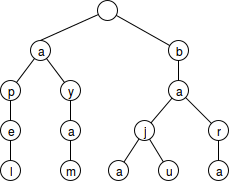
\includegraphics[scale=0.6]{pics/Contoh-StandardTrie}
    \caption{Contoh Standard Trie}
    \label{fig:contoh-standard-trie}
\end{figure}

%-----------------------------------------------------------------------------%
\subsection{Suffix Tree}
%-----------------------------------------------------------------------------% 
\textit{Suffix tree} sering digunakan untuk pencarian sequence yang panjang seperti \textit{genomes} untuk bidang bioinformatik. Pembentukan \textit{suffix tree} mirip seperti \textit{Standard Trie}, namun untuk seluruh \textit{suffix} dalam \textit{string}. Jika diberikan \textit{string} dengan panjang $n$, dibentuk cabang dengan $n(n-1)/2$ \textit{suffix}.  Metode ini banyak dimanfaatkan untuk mempercepat proses pencarian jika diberikan sebuah masukan \textit{query}. Jika terdapat sebuah \textit{pattern} dengan panjang \textit{string} $m$, maka waktu yang dibutuhkan untuk menjalankan proses \textit{pattern matching} adalah $O(dm)$ dengan $d$ adalah ukuran alfabet. Proses pencarian dilakukan dengan menelusuri \textit{path} dari \textit{root} sesuai dengan \textit{sequence query}. Jika seluruh karakter dalam \textit{query} selesai dijalankan, maka proses pencarian berhasil. 

Sebagai contoh \textit{string} 'babaa' menghasilkan \textit{suffix tree} berikut. Jika diberi \textit{query} 'ba' maka akan berhasil terhadap \textit{path} 'babaa' dan 'baa'.
\begin{figure}
    \centering
    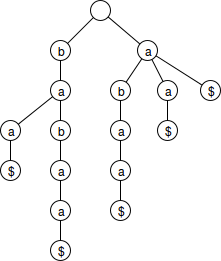
\includegraphics[scale=0.6]{pics/Contoh-SuffixTree}
    \caption{Contoh Suffix Trie}
    \label{fig:contoh-suffix-trie}
\end{figure}

%-----------------------------------------------------------------------------%
%-----------------------------------------------------------------------------%
\section{Semi Supervised}
%-----------------------------------------------------------------------------%
Dalam \textit{machine learning} terdapat dua tipe pendekatan yang umum digunakan yaitu \textit{supervised} dan \textit{unsupervised learning}. Supervised menggunakan data berlabel sebagai data \textit{training} maupun \textit{testing}. Dari kedua data tersebut, dibentuk suatu \textit{classifier} yang dapat memenuhi segala kasus yang mungkin terjadi. Data \textit{testing} digunakan untuk menguji kebaikan \textit{classifier} yang terbentuk. \textit{Unsupervised} menggunakan data yang tidak diberi label sama sekali dan berusaha untuk menemukan pola yang sama untuk suatu kumpulan data tertentu \citep{prakash2014survey}. Pendekatan lain yang merupakan kombinasi antara \textit{supervised} dan \textit{unsupervised learning} adalah \textit{semi supervised learning}. 

\textit{Semi supervised} adalah pendekatan \textit{machine learning} dimana informasi \textit{supervised} data diberikan tidak untuk seluruh data. Sebagian data merupakan data berlabel sementara sebagian lainnya belum memiliki label. Beberapa metode penerapan semi supervised adalah \textit{bootstrapping} (\textit{self training}), \textit{mixture models}, \textit{graph based methods}, \textit{co-training,} dan \textit{multiview learning}.
%(12) MITPress - Semi Supervised Learning

%-----------------------------------------------------------------------------%
\subsection{Bootstrapping}
%-----------------------------------------------------------------------------% 
Model \textit{bootstrapping} merupakan salah satu model \textit{semi supervised learning} yang paling umum digunakan. \textit{Bootstrapping} menggunakan data berlabel berukuran kecil dan data tidak berlabel berukuran jauh lebih besar. Proses anotasi data tidak berlabel dilakukan secara bertahap melalui sejumlah iterasi. Dari data \textit{training} berlabel, dibentuk suatu \textit{classifier} yang kemudian digunakan untuk menganotasi data tidak berlabel. Sejumlah $k$ data baru yang merupakan hasil pelabelan, dimasukkan ke dalam kelompok data berlabel. Proses tersebut dilakukan secara berulang, sehingga semakin lama iterasi jumlah data berlabel akan bertambah. 

Terdapat dua algoritma \textit{bootstrapping} yang pernah digunakan untuk proses \textit{pattern extraction} dan \textit{matching} yaitu \textit{Meta-Bootstrapping} dan \textit{Basilisk} \citep{riloff2003learning}. Keduanya digunakan untuk mengelompokan kata ke dalam suatu kategori semantik jika diberikan korpus teks yang belum dianotasi dan suatu \textit{seed}. \textit{Seed} didefinisikan sebagai korpus kata yang sudah diketahui kategori semantiknya. Secara umum, proses ini akan mencari \textit{pattern} berdasarkan seed yang diberikan. Dari \textit{pattern} yang dihasilkan dan teks yang belum dianotasi, diekstrak entitas baru dan dikelompokan berdasarkan kategori semantiknya. Kata-kata tersebut akan digabungkan ke dalam korpus pasangan kata berelasi.

%-----------------------------------------------------------------------------%
\subsection{Meta Bootstrapping}
%-----------------------------------------------------------------------------% 
Berikut adalah beberapa proses \citep{riloff1999learning} yang dijalankan algoritma \textit{meta bootstrapping} jika diberikan \textit{seed} berukuran kecil yang berasal dari suatu kategori semantik dan korpus yang belum dianotasi.
\begin{enumerate}
  \item Mengekstraksi \textit{pattern} secara otomatis dengan menerapkan syntactic template.
  \item Untuk setiap \textit{pattern} akan diberi bobot berdasarkan jumlah seed yang menghasilkan \textit{pattern}.
  \item Diambil \textit{pattern} terbaik dan seluruh seed lama yang merepresentasikan \textit{pattern} maupun \textit{seed} baru yang berhasil diekstrak disimpan.
  \item Dilakukan pembobotan ulang untuk setiap \textit{pattern} menggunakan \textit{seed} lama dan baru.
\end{enumerate}
Proses diatas dinamakan \textit{mutual bootstrapping} dan setelah proses tersebut selesai, semua entitas baru hasil ekstraksi dievaluasi. Pembobotan entitas baru diberikan berdasarkan jumlah \textit{pattern} yang mengekstrak kata tersebut. Lima kata terbaik diterima dan dimasukkan ke kamus (korpus) kata berelasi untuk selanjutnya diproses ulang.

%-----------------------------------------------------------------------------%
\subsection{Basilisk}
%-----------------------------------------------------------------------------% 
Algoritma \textit{Basilisk} \citep{thelen2002bootstrapping} juga memanfaatkan \textit{pattern} dan \textit{seed} dalam membangun korpus untuk suatu kategori semantik tertentu. Beberapa tahapan yang dijalankan adalah sebagai berikut.
\begin{enumerate}
  \item Secara otomatis membentuk \textit{pattern} dan memberi bobot berdasarkan jumlah seed yang menghasilkan \textit{pattern}. Pattern terbaik dimasukan ke dalam \textit{Pattern Pool}.
  \item Untuk setiap entitas baru yang terekstraksi dari \textit{pattern}, dimasukan ke dalam \textit{Candidate Word Pool}. Pemberian bobot dilakukan berdasarkan jumlah \textit{pattern} yang mengekstraksi dan asosiasi kumulatif kata dengan \textit{seed}.
  \item Sepuluh kata terbaik diambil dan dimasukan ke dalam kamus (korpus) yang kemudian digunakan untuk iterasi selanjutnya. 
\end{enumerate}

Kateogori semantik untuk proses ini bisa lebih dari satu. \textit{Basilisk} memberi bobot berdasarkan informasi kolektif dari kumpulan \textit{pattern} yang mengekstrak kata tersebut. Sementara \textit{Meta-Bootstrapping} hanya mengambil satu \textit{pattern} terbaik dan mengelompokkan seluruh kata yang terekstrak dari \textit{pattern} ke dalam kategori semantik yang sama. Dari hasil penelitian komparatif yang pernah dilakukan \citep{riloff2003learning}, didapatkan \textit{Basilisk} mengungguli performa \textit{Meta-Bootstrapping}. 

%-----------------------------------------------------------------------------%
%-----------------------------------------------------------------------------%
\section{Word Embedding}
%-----------------------------------------------------------------------------%
\textit{Word Embedding} digunakan untuk menentukan similarity antar kata relasi yang dihasilkan dari proses \textit{Pattern Matching}.

%-----------------------------------------------------------------------------%
%-----------------------------------------------------------------------------%
\section{Pointwise Mutual Information}
%-----------------------------------------------------------------------------%
\textit{Pointwise Mutual Information} (PMI) adalah pengukuran nilai asosiasi antar variabel. Dalam bidang \textit{information theory}, PMI dapat dimanfaatkan untuk menghitung asosiasi kemunculan dua buah kata. Jika diberikan dua buah kata $x$ dan $y$, maka nilai PMI kata tersebut dalam suatu dokumen dapat dihitung menggunakan rumus berikut. 
\[ pmi(x;y)=log\frac{p(x,y)}{(x)p(y)}=log\frac{p(x|y)}{p(x)}=log\frac{p(y|x)}{p(y)} \] dengan $p(x)=\frac{f(x)}{N}$
\[ pmi(x;y)=log\frac{f(x)N}{f(x)f(y)} \]
\begin{itemize}
  \item $p(x)$ adalah probabilitas kemunculan kata $x$ dalam korpus
  \item $f(x)$ adalah frekuensi kemunculan kata $x$ dalam korpus
  \item $N$ adalah toatal seluruh kata dalam korpus
\end{itemize}
Pengukuran ini bersifat simetris, sehingga $p(x;y)=p(y;x)$. Nilai PMI dapat merupakan bilangan positif maupun negatif. Jika nilai PMI adalah nol (0), berarti kedua variabel saling \textit{independent}.

%-----------------------------------------------------------------------------%
\subsection{Skip PMI}
%-----------------------------------------------------------------------------% 
PMI umumnya hanya menggunakan model \textit{bigram} atau \textit{trigram}. Model ini hanya melihat hubungan kata yang berdampingan. Sebagai contoh ingin diketahui PMI untuk \textit{bigram} 'hong kong', 'sepak bola', dan 'amerika serikat'. Pada penelitian ini dilakukan modifikasi yaitu membuat model \textit{skip-gram} PMI. Kita menghitung nilai PMI antar dua kata yang dipisahkan dengan $n$ diantaranya. 

%-----------------------------------------------------------------------------%
%-----------------------------------------------------------------------------%
\section{Evaluasi}
%-----------------------------------------------------------------------------%
Evaluasi dilakukan untuk mengetahui kebaikan hasil penelitian. Evaluasi dapat dilakukan dengan mengukur akurasi data yang dihasilkan. Akurasi adalah nilai perbandingan antara jumlah data yang benar dengan jumlah seluruh data (Manning). 
\[ akurasi=\frac{jumlah\,\,data\,\,benar}{jumlah\,\,seluruh\,\,data} \]
Selain menghitung akurasi, proses evaluasi juga menghitung nilai-nilai lainnya. Berikut ada beberapa metode dan teknik evaluasi lain yang digunakan dalam penelitian.

%-----------------------------------------------------------------------------%
\subsection{Sampling}
%-----------------------------------------------------------------------------% 
Terdapat dua kategori utama dalam \textit{sampling} yaitu \textit{probability} dan \textit{non-probability sampling}. Perbedaan utama keduanya adalah pada \textit{probability sampling}, diambil data secara acak (\textit{random}). Dalam \textit{probability sampling}, terdapat beberapa metode yang dapat digunakan seperti \textit{simple random sampling}, \textit{systematic sampling}, \textit{stratified random sampling}, dan \textit{cluster sampling}.
\begin{itemize}
  \item \textit{Simple random sampling} perlu mengetahui seluruh data yang ada dan dari data tersebut dipilih secara acak. Hal ini membuat seluruh data memiliki nilai probabilitas terpilih yang sama. 
  \item \textit{Systematic sampling} memilih setiap data ke-n untuk dijadikan \textit{sample}. 
  \item \textit{Stratified random sampling} akan mengelompokan data ke dalam kategori berdasarkan karakteristik tertentu (strata), kemudian data diambil secara acak dari kategori yang ada. Hal ini menyebabkan hasil lebih representatif. 
  \item \textit{Cluster} sampling mirip seperti \textit{stratified sampling} namun dilakukan jika data kelompok yang ingin di-\textit{sampling} sulit berada di lokasi yang terpisah jauh.
\end{itemize}
Proses \textit{sampling} bermanfaat untuk merepresentasikan data tanpa perlu mengevaluasi seluruh data yang ada. Jika jumlah data yang ingin dievaluasi berukuran besar, proses \textit{sampling} mempercepat pengukuran. Jumlah data yang direpresentasikan oleh satu sample berdasarkan jumlah data asli. Sebagai contoh jika total data adalah 1000 dan jumlah data sample adalah 50, maka satu data \textit{sample} merepresentasikan 20 data asli.
%(Sumber: https://ecduganda.files.wordpress.com/2014/08/how-to-choose-sampling-techniques-for-evaluations.pdf)
%(http://optimierung.mathematik.uni-kl.de/mamaeusch/veroeffentlichungen/ver_texte/sampling_en.pdf)

%-----------------------------------------------------------------------------%
\subsection{Precision dan Recall}
%-----------------------------------------------------------------------------% 
Teknik yang umum digunakan untuk mengevaluasi suatu ekstraksi adalah \textit{precision} dan \textit{recall}. \textit{Precision} adalah nilai yang menyatakan jumlah dokumen benar dan berhasil diambil dibandingkan dengan seluruh jumlah dokumen yang terambil. \textit{Recall} adalah nilai yang menyatakan jumlah dokumen benar dan berhasil diambil dibandingkan dengan jumlah seluruh dokumen yang benar. Semakin banyak dokumen yang diambil maka nilai \textit{recall} akan meningkat sementara nilai \textit{precision} cenderung menurun. 

%-----------------------------------------------------------------------------%
\subsection{Kappa}
%-----------------------------------------------------------------------------%  
Nilai kappa ($\kappa$) merepresentasikan tingkat persetujuan antar anotator. Kappa digunakan pada penelitian yang menggunakan bantuan anotator untuk memberi penilaian secara manual. Peniliaian didapatkan menggunakan rumus berikut.
\[ \kappa=\frac{P(A)-P(E)}{1-P(E)} \]
\begin{itemize}
  \item $P(A)$ adalah proporsi penilaian yang setuju (\textit{agreement})
  \item $P(E)$ adalah proporsi penilaian yang kebetulan
\end{itemize}
\cite{landis1977measurement} mendefiniskan tingkat persetujuan berdasarkan nilai Kappa yang diperoleh. 
\begin{table}
  \centering
    \caption{Skala pengukuran Kappa}
    \label{table:skalaKappa}
    \begin{tabular}{|c|c|}
      \hline
      Statistik Kappa & Tingkat persetujuan \\ \hline
      < 0.00 & \textit{Poor} \\ \hline
      0.00 - 0.20 & \textit{Slight} \\ \hline
      0.21 - 0.40 & \textit{Fair} \\ \hline
      0.41 - 0.60 & \textit{Moderate} \\ \hline
      0.61 - 0.80 & \textit{Substantial} \\ \hline
      0.81 - 1.00 & \textit{Almost Perfect} \\ \hline
    \end{tabular}
\end{table}

Beberapa variasi perhitungan untuk Kappa adalah Cohen's Kappa dan Fleiss' Kappa. Cohen's Kappa digunakan untuk mengukur tingkat persetujuan antar dua anotator. Jika diberikan data dengan $n$ label dan $m_ij$ merepresentasikan jumlah data yang diberi label $i$ oleh anotator pertama dan label $j$ oleh anotator kedua, maka proses perhitungan $P(A)$ dan $P(E)$ untuk Cohen's Kappa adalah sebagai berikut.
\[ P(A)=\frac{\sum_{k=1}^{n} m_kk}{total\,\,data} \]
\[ P(E)=\frac{\sum_{k=1}^{n} ( \sum_{j=1}^{n} m_kj . \sum_{i=1}^{n} m_ik ) }{total\,\,data} \]

Fleiss' Kappa mengukur tingkat persetujuan antar sekelompok anotator berjumlah lebih dari dua. Jika diberikan $N$ data dengan $n$ anotator dimana setiap data diantosi ke dalam salah satu dari $k$ kategori dan $n_ij$ merepresentasikan total anotator yang memberi data $i$ ke label $j$, proses perhitungan $P(A)$ dan $P(E)$ untuk Fleiss' Kappa adalah sebagai berikut.
\[ P(A)=\frac{1}{N}\sum_{i=1}^{N}P_i \:\:\:\:\:dengan\:\:\:\:\: P_i=\frac{1}{n(n-1)}[(\sum_{j=1}^{k}n^2_ij)-(n)] \]


%-----------------------------------------------------------------------------%
\subsection{Spearman's Rho}
%-----------------------------------------------------------------------------% 
\textit{Spearman's rank correlation coefficient} adalah nilai koefisien korelasi antar \textit{ranking} dua parameter. Nilai \textit{Spearman correlation} sama dengan nilai \textit{Pearson correlation} antar dua paramter yang telah di-\textit{ranking}. \textit{Pearson correlation}  menggambarkan nilai linear antara dua parameter. \textit{Spearman correlation} berkisar antara $-1$ hingga $+1$.

Spearman's rho adalah nilai Pearson Correlation Coefficient antar dua variabel yang telah di-\textit{ranking}. Untuk mendapatkan nilai koefisien ($r_s$), menggunakan rumus berikut.
\[ r_s = \rho_{rg_X,rg_Y} = \frac{cov(rg_X,rg_Y)}{\sigma_{rg_X}\sigma_{rg_Y}} \]
\begin{itemize}
  \item $\rho$ adalah \textit{Pearson correlation coefficent} yang diaplikasikan pada variabel \textit{ranking}
  \item $cov(rg_X,rg_Y)$ adalah nilai \textit{covariance} antar variabel \textit{ranking}
  \item $\sigma_{rg_X}$ dan $\sigma_{rg_Y}$ adalah nilai standard deviasi variabel \textit{ranking}
\end{itemize}
Jika seluruh \textit{ranking} berbeda, proses komputasi dapat dilakukan menggunakan rumus berikut.
\[ r_s = 1-\frac{6 \Sigma d_i^2}{n(n^2-1)} \]
\begin{itemize}
  \item $d_i = rg(X_i)-rg(Y_i)$ adalah selisih antara dua \textit{ranking}
  \item $n$ adalah jumlah observasi
\end{itemize}

%-----------------------------------------------------------------------------%
\chapter{\babTiga}
%-----------------------------------------------------------------------------%
Pada bab ini dipaparkan mengenai rancangan dan tahap-tahap proses ekstraksi relasi semantik, mulai dari rancangan pengembangan korpus, pembentukan \textit{seed}, pembentukan \textit{pattern}, ekstraksi \textit{pair}, \textit{cycle semi-supervised}, dan strategi evaluasi yang dilakukan untuk pasangan kata relasi Bahasa Indonesia. 


%-----------------------------------------------------------------------------%
\section{Rancangan Pengembangan Korpus}
%-----------------------------------------------------------------------------%
Penelitian ini mengusulkan pembangunan korpus pasangan kata berelasi menggunakan arsitektur yang dapat dilihat pada gambar \ref{fig:arsitektur-penelitian}. Terdapat dua sumber data utama yang digunakan yaitu WordNet Bahasa untuk pembentukan \textit{seed} dan artikel Wikipedia Bahasa Indonesia sebagai korpus teks. Secara garis besar, terdapat beberapa tahap yang perlu dilakukan yaitu pengumpulan \textit{seed}, \textit{pre-processing} data Wikipedia, \textit{sentence tagging}, \textit{pattern extraction}, \textit{pattern matching}, dan terakhir adalah evaluasi. Untuk proses \textit{sentence tagging}, \textit{pattern extraction}, dan \textit{pattern matching} dilakukan secara berulang sesuai dengan metode \textit{bootstrapping}. 

\begin{figure}
    \centering
    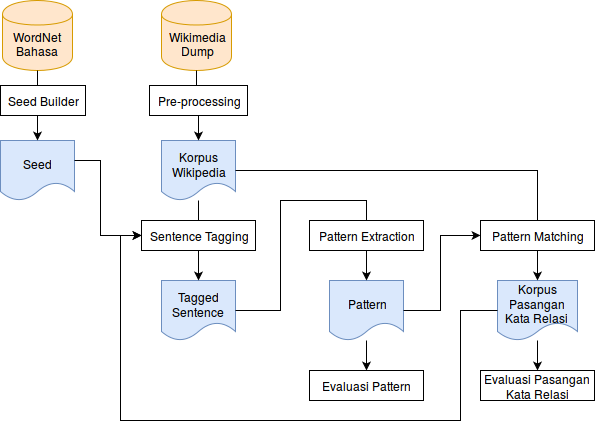
\includegraphics[scale=0.55]{pics/Pic01-SemiSupervisedCycle}
    \caption{Arsitektur Penelititan}
    \label{fig:arsitektur-penelitian}
\end{figure}

\noindent Berikut adalah penjelasan singkat setiap tahapan pada gambar di atas.
\begin{enumerate}
  \item \textit{Pre-processing} data \\
  Sebelum memulai penelitian, terdapat dua hal utama yang perlu dilakukan yaitu pengumpulan \textit{seed} dan pembentukan kalimat Wikipedia. Pengumpulan \textit{seed} dilakukan untuk mendapatkan pasangan kata relasi yang digunakan sebagai dasar penelitian. Proses ini memanfaatkan \textit{resource} yang dimiliki WordNet Bahasa. Selanjutnya, artikel Wikipedia yang diperoleh dalam bentuk \textit{Wikipedia dump} perlu diolah sehingga memiliki representasi sesuai dengan format yang diharapkan. Informasi yang diperlukan hanya bagian isi artikel dan ditulis dalam bentuk kalimat untuk setiap baris.
  \item Pembentukan \textit{pattern} \\
  Menggunakan \textit{seed} dan korpus kalimat Wikipedia, dilakukan \textit{tagging} pasangan kata berelasi terhadap kalimat-kalimat yang ada. Kalimat yang mengandung pasangan kata berelasi akan ditandai dan disimpan sebagai dasar proses selanjutnya. Kalimat-kalimat yang sudah di-\textit{tag} dengan pasangan kata berelasi kemudian akan digunakan untuk proses \textit{pattern extraction}. Hasil dari proses ini adalah sejumlah \textit{pattern} leksikal terbaik dari banyak \textit{pattern} unik yang dihasilkan.
  \item Ektraksi pasangan kata relasi \\
  \textit{Pattern} yang dihasilkan digunakan untuk mengekstrak pasangan kata relasi baru dengan dibantu korpus Wikipedia dengan \textit{POS tag}. Proses \textit{pattern matching} dilakukan dengan mencocokkan kata-kata bebas dalam \textit{pattern} dengan kalimat, kemudian mengambil bagian yang menempati posisi \textit{tag} hipernim-hiponim. Pasangan kata yang dihasilkan masuk ke dalam korpus pasangan kata relasi hipernim-hiponim.
  \item \textit{Cycle semi-supervised} \\ 
  Korpus pasangan kata relasi yang terbentuk digunakan untuk iterasi selanjutnya sesuai dengan metode \textit{bootstrapping}. Proses iterasi dilakukan hingga jumlah pasangan kata relasi baru yang dihasilkan jenuh. Setelah satu eksperimen selesai, proses evaluasi dilakukan secara kolektif untuk mengetahui akurasi setiap data yang dihasilkan.
\end{enumerate}

\noindent Proses ini diharapkan dapat menghasilkan korpus pasangan kata relasi \textit{hyponym-hypernym} yang berkualitas baik dan berukuran besar.


%-----------------------------------------------------------------------------%
\section{Pre-processing Data}
%-----------------------------------------------------------------------------%
Proses inti dari penelitian ini, \textit{pattern extraction} dan \textit{matching}, memerlukan dua masukan utama yaitu sejumlah pasangan kata hipernim-hiponim (\textit{seed}) dan teks dokumen yang digunakan sebagai korpus. Pasangan kata hipernim-hiponim digunakan untuk proses pembentukan \textit{pattern} sementara teks dokumen digunakan untuk memperoleh pasangan kata baru. Karena belum ada korpus pasangan kata relasi hipernim-hiponim Bahasa Indonesia, perlu dibentuk \textit{seed} yang akan digunakan sebagai dasar pasangan kata hipernim-hiponim. Teks dokumen yang digunakan, yaitu Wikipedia, juga memerlukan pemrosesan sebelum menjadi masukan sistem.

%-----------------------------------------------------------------------------%
\subsection{Pembentukan Kalimat Wikipedia}
%-----------------------------------------------------------------------------%
Data Wikipedia yang diperoleh dari Wikimedia \textit{dumps} masih mengandung banyak \textit{tag} yang tidak digunakan pada penelitian ini seperti \textit{tag} \textit{id} dan \textit{revision}. Selain itu simbol-simbol khusus (\textit{markup}). Penelitian ini ingin mengekstrak \textit{pattern} dari \textit{free text}, sehingga format-format khusus tersebut perlu dibersihkan. Gambar \ref{fig:wiki-dump} menunjukkan contoh data XML yang diperoleh dari Wikimedia Dump. Setelah data Wikipedia dibersihkan dari simbol-simbol tersebut, langkah selanjutnya adalah merepresentasikan korpus dalam bentuk kalimat. 

\begin{figure}
    \centering
    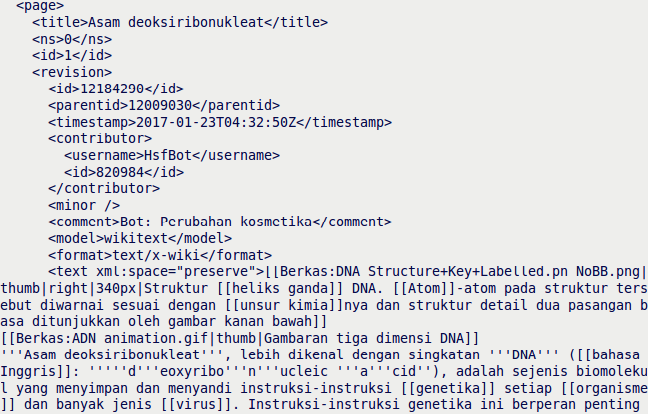
\includegraphics[width=\linewidth]{pics/WikipediaDump}
    \caption{Data XML Wikipedia Dump}
    \label{fig:wiki-dump}
\end{figure}

Artikel-artikel Wikipedia dibentuk ke dalam format yang telah didefinisikan dengan satu kalimat dipisahkan untuk setiap barisnya. Selanjutnya, data akan di format ulang sesuai definisi untuk mempermudah pemrosesan selanjutnya. Beberapa aturan yang diberikan adalah menghilangkan frasa di dalma tanda kurung, menghilangkan simbol, serta memberi \textit{tag start} dan \textit{end} pada awal dan akhir kalimat.

\begin{figure}
    \centering
    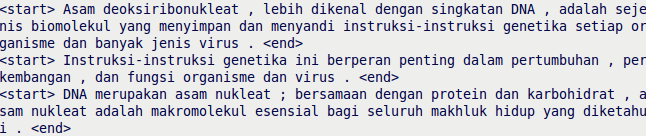
\includegraphics[width=\linewidth]{pics/kalimatWiki}
    \caption{Korpus kalimat Wikipedia tanpa \textit{POS tag}}
    \label{fig:kalimat-wiki}
\end{figure}

\begin{figure}
    \centering
    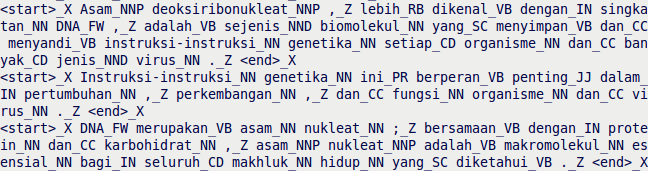
\includegraphics[width=\linewidth]{pics/kalimatWikiTag}
    \caption{Korpus kalimat Wikipedia \textit{POS tag}}
    \label{fig:kalimat-wiki-tag}
\end{figure}

\noindent Korpus kalimat yang dihasilkan kemudian digunakan untuk proses \textit{part-of-speech tagging}. Hasil dari \textit{pre-processing} data Wikipedia adalah dua korpus besar yaitu korpus kalimat tanpa \textit{POS tag} (Gambar \ref{fig:kalimat-wiki}) yang digunakan sebagai masukan \textit{pattern extraction} dan korpus kalimat dengan \textit{POS tag} (Gambar \ref{fig:kalimat-wiki-tag}) yang digunakan sebagai masukan \textit{pattern matching}. 

%-----------------------------------------------------------------------------%
\subsection{Pengumpulan Seed}
%-----------------------------------------------------------------------------%
Pengumpulan pasangan kata awal (\textit{seed}) dilakukan karena Bahasa Indonesia belum memiliki korpus tersebut, sementara data diperlukan sebagai pengetahuan awal untuk proses selanjutnya. Pasangan kata relasi hipernim-hiponim diambil dari data yang dimilki oleh WordNet Bahasa yang dikembangkan oleh NTU. Pemanfaatan WordNet Bahasa dilatarbelakangi jumlahnya yang lebih besar dibanding Indonesian WordNet (IWN). Relasi semantik antar kata pada WordNet Bahasa memanfaatkan WordNet Princeton versi 3.0. \textit{Synset} pada WordNet Bahasa dipetakan ke \textit{synset} WordNet Princeton, sehingga relasi semantik yang dimiliki oleh WordNet Princeton ikut diwarisi. Alasan lain penggunaan WordNet Bahasa adalah karena telah terintegrasi dengan \textit{tools} nltk sehingga dapat langsung digunakan untuk membentuk \textit{seed} secara mudah.

Seluruh lema Bahasa Indonesia yang ada di dalam korpus WordNet Bahasa diambil. Untuk setiap lema, akan dicari hipernimnya sehingga dapat dibentuk menjadi pasangan kata relasi hipernim-hiponim. Sayangnya, tidak semua pasangan kata yang dihasilkan adalah benar akibat beberapa kekurangan yang dimiliki WordNet Bahasa. Untuk itu dilakukan proses filterisasi untuk meminimalisasi \textit{error} yang mungkin terjadi. Dua tipe filterisasi yang digunakan adalah filterisasi lema sama dan filterisasi \textit{strict}. Filterisasi lema sama memperbolehkan pasangan kata terbentuk dari kata dengan \textit{synset} hiperim berbenda namun memiliki sejumlah lema yang sama. Sementara filterisasi \textit{strict} tidak memperbolehkan hal tersebut. Seluruh pasangan kata yang lolos proses filterisasi dibentuk menjadi \textit{tuple} biner. Hasil akhir dari proses ini adalah himpunan \textit{tuple} yang berisi dua elemen dengan format $(w_1;w_2)$ dimana $w_1$ pertama merupakan kata hiponim dan $w_2$ merupakan kata hipernimnya.

Beberapa contoh \textit{seed} yang dihasilkan adalah `(novel;buku)', `(salmon;ikan)', `(humus;tanah)', `(oktan;ukuran)', dan `(kucai;sayuran)'.


%-----------------------------------------------------------------------------%
\section{Pembentukan Pattern}
%-----------------------------------------------------------------------------%
\textit{Pattern} leksikal yang akan digunakan ingin seluruhnya dibentuk secara otomatis oleh sistem. Terdapat dua masukan utama untuk proses ini yaitu pasangan kata relasi hipernim-hiponim yang telah diketahui dan korpus dokumen. Pada tahap awal, pasangan kata relasi masukan adalah \textit{seed} yang dibentuk menggunakan WordNet Bahasa. Untuk tahap selanjutnya, pasangan kata relasi menggunakan korpus \textit{pair} hasil proses ekstraksi. Terdapat dua tahapan utama dalam pembentukan \textit{pattern} yaitu \textit{sentence tagging} dan \textit{pattern extraction}.

%-----------------------------------------------------------------------------%
\subsection{Sentence Tagging}
%-----------------------------------------------------------------------------%
\textit{Sentence tagging} adalah proses \textit{intermediate} yang perlu dilakukan sebelum sistem dapat membentuk sebuah \textit{pattern} leksikal. Proses ini akan memberi \textit{tag} hipernim dan hiponim terhadap suatu kata di dalam kalimat. Masukan untuk proses ini adalah pasangan kata relasi dan korpus Wikipedia tanpa \textit{POS tag}. Untuk setiap kalimat dalam korpus Wikipedia, dicek apakah kalimat tersebut mengandung pasangan kata relasi. Jika mengandung, maka kata dalam kalimat yang merupakan pasangan kata akan di-\textit{tag} hipernim dan hiponim. Satu kalimat dicocokan dengan seluruh pasangan kata relasi karena terdapat kasus dimana satu kalimat mengandung lebih dari satu pasangan kata relasi. Proses ini menghasilkan kalimat-kalimat Wikipedia yang telah diberi \textit{tag} hipernim atau hiponim.

Sebagai contoh, terdapat pasangan kata `(sepak bola;olahraga)' serta kalimat `{\tagStart} sepak bola adalah cabang olahraga yang menggunakan bola berbahan kulit dan dimainkan oleh dua tim . {\fontfamily{qcr}\selectfont<end>}'. Kalimat dengan tag hipernim-hiponim yang dihasilkan adalah `{\tagStart} {\tagHyponym}sepak bola{\tagHyponymEnd} adalah cabang {\tagHypernym}olahraga{\tagHypernymEnd} yang menggunakan bola berbahan kulit dan dimainkan oleh dua tim . {\tagEnd}'. Dengan adanya penanda kata mana yang merupakan hipernim dan hiponim, proses ekstraksi \textit{pattern} akan lebih mudah dilaksanakan.

%-----------------------------------------------------------------------------%
\subsection{Pattern Extraction}
%-----------------------------------------------------------------------------%
Setelah didapatkan kumpulan kalimat yang sudah diberi \textit{tag} hipernim dan hiponim, dicari barisan kata yang mirip dan dapat dijadikan sebuah \textit{pattern}. \textit{Pattern extraction} adalah proses untuk mendapatkan \textit{pattern} leksikal yang kemunculannya sering dalam korpus. Masukan dari proses ini adalah kalimat-kalimat Wikipedia yang telah diberi \textit{tag} hipernim dan hiponim. Dari kalimat tersebut akan dibuat suatu \textit{pattern tree} yang merepresentasikan seluruh \textit{pattern} leksikal yang ditemukan dan digunakan untuk mendapatkan \textit{pattern} yang paling sering muncul. Namun, tidak seluruh kata dalam kalimat akan dimasukkan ke dalam \textit{pattern tree}. Hanya bagian-bagian yang dianggap relevan saja yang digunakan untuk proses \textit{pattern extraction}. Pada tahap awal pengembangan, pemanfaatan seluruh kata dalam kalimat menghasilkan \textit{pattern} yang sangat banyak dan tidak umum. Sebagai contoh, proses \textit{sentence tagging} menghasilkan tiga kalimat yang telah diberi \textit{tag} hipernim-hiponim berikut. Kalimat digunakan untuk mencari \textit{pattern} yang merepresentasikan relasi hipernim-hiponim.
\begin{itemize}
  \item {\tagStart} {\tagHyponym}kelinci{\tagHyponymEnd} adalah {\tagHypernym}binatang{\tagHypernymEnd} yang gemar memakan wortel . {\tagEnd}
  \item {\tagStart} {\tagHyponym}mobil{\tagHyponymEnd} adalah {\tagHypernym}kendaaraan{\tagHypernymEnd} beroda empat . {\tagEnd}
  \item {\tagStart} selain sepak bola, {\tagHyponym}basket{\tagHyponymEnd} adalah {\tagHypernym}olahraga{\tagHypernymEnd} yang disukai masyarakat . {\tagEnd}
\end{itemize}
Dari kumpulan kalimat di atas, \textit{pattern} yang diinginkan untuk terbentuk adalah `{\tagHyponym} adalah {\tagHypernym}'. Sementara bagian seperti `gemar memakan wortel', `beroda empat', dan `yang disukai masyarakat' tidak merepresentasikan \textit{pattern} hipernim-hiponim. Hal tersebut memperlihatkan bahwa tidak seluruh kata dalam kalimat perlu dimasukkan ke dalam \textit{pattern tree}.

Berdasarkan hasil pengamatan kualitatif dari sejumlah kalimat yang telah diberi \textit{tag} hipernim-hiponim, terdapat tiga tipe pendekatan yang digunakan untuk proses pembentukan \textit{pattern}. Bagian dalam kalimat yang diperhatikan untuk pembuatan \textit{pattern} adalah kata diantara dua \textit{tag} hipernim-hiponim, $n$ kata sebelum \textit{tag} pertama, dan $n$ kata setelah \textit{tag} terakhir. Bagian kata yang diambil akan dimasukkan ke dalam \textit{pattern tree} untuk diketahui kemunculannya yang paling sering. Seluruh \textit{pattern} dapat direpresentasikan menjadi vektor dan diurutkan berdasarkan bobot tertingginya. Proses ini akan menghasilkan kumpulan \textit{pattern} unik yang terurut berdasarkan bobotnya. Dari \textit{pattern} unik tersebut, akan diambil sejumlah \textit{pattern} terbaik untuk kemudian digunakan sebagai dasar pembentukan \textit{pair} baru. Lebih rinci mengenai proses pembentukan \textit{pattern} dapat dilihat pada bab 4.4.
%
% Sebagai contoh terdapat beberapa kalimat berikut.
% \begin{itemize}
%   \item {\tagStart} {\tagHyponym}piano{\tagHyponymEnd} adalah {\tagHypernym}alat musik{\tagHypernymEnd} yang dimainkan dengan cara dipukul . {\tagEnd}
%   \item {\tagStart} {\tagHyponym}komputer{\tagHyponymEnd} adalah {\tagHypernym}alat{\tagHypernymEnd} yang dipakai untuk mengolah data . {\tagEnd}
%   \item {\tagStart} {\tagHyponym}tupai{\tagHyponymEnd} adalah {\tagHypernym}mamalia{\tagHypernymEnd} yang mirip dengan bajing . {\tagEnd}
% \end{itemize}
%\noindent Dari kalimat di atas \textit{pattern} unik yang dihasilkan yaitu `{\tagHyponym} adalah {\tagHypernym}'. 


%-----------------------------------------------------------------------------%
\section{Ekstraksi Pair}
%-----------------------------------------------------------------------------%
Tujuan utama dari penelitian ini adalah membentuk korpus pasangan kata relasi, sehingga proses ekstraksi \textit{pair} adalah tahapan utama dari keseluruhan penelitian. Pada proses ini, dimanfaatkan \textit{pattern} yang telah terbentuk sebelumnya untuk mengekstrak pasangan kata baru. Pasangan kata tersebut kemudian difilter sebelum digabung ke dalam korpus pasangan kata relasi. Ektraksi \textit{pair} menggunakan teknik \textit{pattern matching}. Selanjutnya \textit{pair} akan diberi bobot dan hanya \textit{pair} yang bobotnya memenuhi nilai \textit{treshold}-lah yang akan dimasukkan dalam korpus pasangan kata relasi.

%-----------------------------------------------------------------------------%
\subsection{Pattern Matching}
%-----------------------------------------------------------------------------%
\textit{Pattern matching} adalah proses mencocokkan suatu \textit{pattern} ke dalam teks dokumen. Proses ini dilaksanakan untuk mendapatkan pasangan kata relasi (\textit{pair}) baru. Dua masukan utama untuk proses ini adalah \textit{pattern} dan korpus Wikipedia \textit{POS tag}. Penggunaan korpus Wikipedia dengan \textit{POS tag} untuk membatasi \textit{pair} yang terekestrak hanya berasal dari kelas kata benda, \textit{noun} (NN) atau \textit{proper noun} (NNP). Pemilihan POS \textit{tag} yang digunakan berdasarkan didefinisikan yang dibuat oleh \cite{dinakaramani2014designing}. Sementara, hanya memperhatikan kata benda karena relasi hipernim-hiponim umumnya digunakan untuk antar kelas kata tersebut. Penelitian ini juga merupakan penelitian awal ekstraksi pasangan kata relasi hipernim-hiponim, sehingga diputuskan untuk fokus pada kata benda saja. 

Pada masa awal pembangunan sistem \textit{pattern matching}, tidak seluruh \textit{pair} yang dihasilkan benar memiliki relasi hipernim-hiponim. Untuk itu, dihitung nilai bobot untuk seluruh \textit{pair} yang dihasilkan. Nilai bobot digunakan untuk dibandingkan dengan nilai threshold yang didefinisikan. Hanya \textit{pair} yang bobotnya melebihi nilai \textit{threshold} yang dapat masuk ke korpus pasangan kata relasi.

Sebagai contoh, terdapat \textit{pattern} leksikal `{\tagHyponym} adalah {\tagHypernym} yang'. Berikut adalah beberapa kalimat Wikipedia dengan \textit{POS tag}.

\begin{itemize}
  \item {\tagStart}\_X sepak\_NNP bola\_NNP adalah\_VB olahraga\_NN paling\_RB populer\_JJ di\_IN Britania\_NNP .\_Z {\tagEnd}\_X
  \item {\tagStart}\_X Berikut\_VB adalah\_VB daftar\_NN penghargaan\_NN yang\_SC diberikan\_VB .\_Z {\tagEnd}\_X
  \item {\tagStart}\_X Gado-gado\_NNP adalah\_VB makanan\_NN yang\_SC berasal\_VB dari\_IN Betawi\_NN .\_Z {\tagEnd}\_X
\end{itemize}

\textit{Pair} yang dihasilkan setelah melalui tahap \textit{pattern matching} hanya `(gado-gado;makanan)'. Pasangan kata `(berikut;daftar penghargaan)' tidak termasuk karena kata `berikut' bukan merupakan kata benda (\textit{noun}). Sementara walau `(sepak bola;olahraga)' adalah pasangan kata hipernim-hiponim yang benar, kalimat tersebut tidak cocok dengan \textit{pattern} leksikal yang diberikan menyebabkan \textit{pair} tidak terekstrak. Lebih rinci mengenai proses ekstraksi \textit{pair} dapat dilihat pada bab 4.5.

%-----------------------------------------------------------------------------%
\subsection{Pembobotan dan Filterisasi}
%-----------------------------------------------------------------------------%
Kumpulan \textit{pair} yang berhasil terekstrak tidak seluruhnya diterima ke dalam korpus pasangan kata relasi. Hanya \textit{pair} yang diyakini benar yang dapat masuk, untuk itu perlu dilakukan proses filterisasi. Setiap \textit{pair} akan diberi bobot dimana nilai bobot suatu \textit{pair} dihitung berdasarkan fitur-fitur yang dimiliki yang disimpan dalam bentuk vektor. Bobot suatu \textit{pair} dapat dianggap sebagai nilai \textit{confidence} apakah benar \textit{pair} tersebut memiliki relasi hipernim-hiponim. 

Informasi utama dalam menghitung bobot suatu \textit{pair} adalah jumlah \textit{pattern} yang membentuk \textit{pair} tersebut serta nilai \textit{similariy} antara dua kata dalam \textit{pair}. Perhitungan jumlah \textit{pattern} pembentuk \textit{pair} dilakukan pada tahap \textit{pattern matching}. Sementara nilai \textit{similarity} dihitung menggunakan model \textit{word embedding}. Pemilihan informasi tersebut berdasarkan pengamatan kualitatif dari vektor \textit{pair} yang dihasilkan. Setiap \textit{pair} yang nilai bobotnya melebih nilai \textit{threshold} yang didefinisikan dapat masuk ke dalam korpus pasangan kata relasi. Proses pembobotan merupakan usulan dalam penelitian ini sehingga belum dapat dikatakan yang terbaik karena juga masih ditemukan \textit{pair} yang tidak lolos filterisasi namun benar berelasi hipernim-hiponim.


%-----------------------------------------------------------------------------%
\section{Cycle Semi-Supervised}
%-----------------------------------------------------------------------------%
Pembelajaran menggunakan pendekatan \textit{semi supervised learning} dilatarbelakangi ketersediaan pasangan kata relasi semantik yang telah diketahui (\textit{seed}) berukuran terbatas dan korpus berukuran besar yang belum dianotasi. Ingin didapatkan \textit{pair} baru dari korpus yang belum diantoasi tersebut. Metode \textit{semi supervised} yang diterapkan adalah \textit{Bootstrapping}. Untuk lebih spesifiknya, algoritma \textit{bootstrapping} yang digunakan gabungan antara Meta-Bootstrapping dan Basilisk dengan beberapa modifikasi. Pemilihan metode tersebut didasari proses ekstraksi \textit{pair} baru yang memanfaatkan \textit{pattern}. Secara umum, proses \textit{bootstrapping} dikelompokan ke dalam dua tahap yaitu iterasi pertama dan iterasi ke-2 hingga n.

Pada iterasi pertama, proses pembentukan \textit{pattern} memanfaatkan \textit{seed} yang berasal dari WordNet Bahasa. Tahap \textit{pre-processing} menghasilkan kumpulan \textit{seed} dan korpus kalimat Wikipedia. \textit{Seed} digunakan untuk \textit{tagging} kalimat Wikipedia sehingga menghasilkan kalimat yang telah di-\textit{tag} hipernim-hiponim. Kalimat-kalimat tersebut digunakan untuk membentuk \textit{pattern} unik yang digunakan untuk memulai iterasi \textit{semi supervised}. \textit{Pattern} yang dibentuk dari filterisasi \textit{seed} lema sama maupun \textit{strict} digabung dan diurutkan berdasarkan bobot yang dimiliki. Lima \textit{pattern} terbaik diambil untuk selanjutnya digunakan dalam proses ekstraksi \textit{pair}. Sementara \textit{seed} yang membentuk kelima \textit{pattern} tersebut langsung dimasukkan ke dalam korpus pasangan relasi kata. Hal tersebut dilakukan untuk memfilter \textit{seed} salah yang terbentuk akibat \textit{error} dari \textit{resource} WordNet Bahasa. Selanjutnya, \textit{pattern} digunakan untuk mengekstrak \textit{pair} baru dan melakukan pembobotan terhadap \textit{pair}. Seluruh \textit{pair} yang nilai bobotnya melebihi \textit{threshold} bergabung dengan \textit{pair} dalam korpus pasangan kata relasi.

Iteriasi selanjutnya mirip seperti iterasi pertama yaitu melakukan \textit{tagging} pasangan kata relasi terhadapa korpus kalimat Wikipedia. Namun, untuk iterasi ke-2 hingga selanjutnya, pasangan kata yang digunakan untuk proses \textit{tagging} adalah dari korpus pasangan kata relasi semantik yang dihasilkan. Setelah mendapatkan kalimat yang telah di-\textit{tag} hipernim-hiponim, dilanjutkan dengan proses \textit{pattern extraction}. \textit{Pattern} yang dihasilkan akan digabung dengan seluruh \textit{pattern} lama kemudian diurutkan. Seperti pada metode \textit{Basilisk}, jumlah \textit{pattern} yang digunakan pada iterasi berikutnya akan bertambah. Satu \textit{pattern} terbaik dari hasil pengurutan bergabung dengan \textit{pattern} terpilih lama untuk digunakan dalam proses \textit{pattern matching}. Hal ini membuka kemungkinan adanya \textit{pair} baru terekstrak. Sama seperti proses sebelumnya, \textit{pair} yang bobotnya melebihi nilai \textit{threshold} digabung ke dalam \noindent pasangan kata relasi.

Iterasi dilakukan hingga korpus pasangan kata relasi jenuh atau dapat dikatakan \textit{pair} baru yang masuk ke dalam korpus berjumlah sedikit. Pada penelitian ini, jika \textit{pair} baru berjumlah kurang dari lima puluh maka iterasi akan berhenti. Evaluasi \textit{pattern} dan \textit{pair} dilakukan secara kolektif diakhir eksperimen. Anotator melakukan evaluasi secara manual untuk mengetahui kualitas \textit{pattern} dan \textit{pair} yang dihasilkan.


%-----------------------------------------------------------------------------%
\section{Metode Evaluasi}
%-----------------------------------------------------------------------------%
Penelitian ini tidak hanya menghasilkan korpus pasangan kata relasi hipernim-hiponim, namun juga \textit{pattern} leksikal Bahasa Indonesia yang merepresentasikan relasi tersebut. Setelah suatu eksperimen selesai, evaluasi dilakukan terhadap \textit{pattern} dan \textit{pair} yang dihasilkan. Proses evaluasi dilakukan dengan bantuan anotator.

%-----------------------------------------------------------------------------%
\subsection{Evaluasi Pair}
%-----------------------------------------------------------------------------%
Evaluasi \textit{pair} dilakukan menggunakan teknik \textit{random sampling}. Sejumlah \textit{pair} yang dihasilkan diambil secara acak dan dianotasi dengan nilai 'benar' atau 'salah' oleh anotator. Berikut adalah proses dalam evaluasi \textit{pair} hasil ekstraksi:
\begin{enumerate}
  \item Terdapat tiga anotator berbeda yang menganotasi data yang sama. 
  \item Anotator memberi nilai benar atau salah terhadap suatu \textit{pair} serta kategori yang didefinisikan. Untuk \textit{pair} benar dapat termasuk kategori \textit{pair} adalah \textit{instance-class} atau \textit{pair} adalah \textit{class-class}. Untuk \textit{pair} salah dapat termasuk kategori \textit{pair} tanpa relasi, \textit{pair} dengan relasi semantik lain, atau \textit{pair} yang posisi hypernym-hyponym-nya terbalik. 
  \item Nilai Kappa dihitung untuk mengetahui tingkat persetujuan antar anotator. Perhitungan dilakukan menggunakan Fleiss' Kappa.
  \item Hasil anotasi digunakan untuk menghitung akurasi \textit{pair} yang dihasilkan sistem.
\end{enumerate}

% TODO: tambahin penjelasan instance-class di bab 2 !!!
Dari setiap nilai anotasi, \textit{pair} dimasukkan ke dalam kategori yang lebih spesifik. Untuk data yang dianotasi benar, \textit{pair} dapat dimasukkan ke dalam dua kategori yaitu \textit{instance-class} atau \textit{class-class}. \textit{pair} dimasukkan ke dalam kategori instance-class jika kata hyponym merupakan suatu instance, sementara kategori class-class jika kata hyponym merupakan suatu class. Untuk data bernilai salah, dapat dimasukkan ke kategori salah tanpa hubungan, salah akibat posisi hiponim-hipernim terbalik (\textit{false posistion}), atau salah dengan relasi semantik lain (\textit{false relation}). Kategori salah akibat posisi hiponim-hipernim terbalik terjadi saat kedua kata yang terekstrak benar memiliki relasi semantik hiponim-hipernim namun kata yang menempati posisi hiponim seharusnya adalah hipernim, begitu pula sebaliknya. Suatu \textit{pair} dapat digolongkan ke dalam kategori salah dengan relasi semantik lain jika kedua kedua kata dalam \textit{pair} tidak berhubungan hipernim-hiponim, namun memiliki relasi lain. Dalam penelitian ini, relasi lain hanya khusus dalam relasi semantik sinonim, antonim, atau meronym-holonym.

Akurasi \textit{pair} dihitung dengan melihat label benar atau salah yang diberikan oleh anotator. Jika terdapat perbedaan anotasi maka dilakukan \textit{voting} untuk menentukan label apa yang dipilih. Nilai akurasi dilihat terhadap seluruh eksperimen maupun setiap \textit{pattern} yang digunakan.
% Terdapat dua akurasi yang akan dihitung untuk setiap iterasi yaitu akurasi sampel dan akurasi total. Setiap iterasi menghasilkan \textit{pair} baru dan dari \textit{pair} baru tersebut diambil sampel untuk dianotasi. Nilai akurasi sampel adalah perbandingan antara data sampel baru benar dengan total data sampel baru. 
% \begin{equation}
% akurasi\,\,sampel = \frac{jumlah\,\,data\,\,sampel\,\,baru\,\,benar}{jumlah\,\,sampel\,\,baru}
% \end{equation}

% \noindent Sementara, akurasi total adalah perbandingan antara total data sampel bener dengan total data sampel.
% \begin{equation}
% akurasi\,\,total = \frac{jumlah\,\,total\,\,sampel\,\,benar}{jumlah\,\,total\,\,sampel}
% \end{equation}

%-----------------------------------------------------------------------------%
\subsection{Evaluasi Pattern}
%-----------------------------------------------------------------------------%
Evaluasi \textit{pattern} dilakukan dengan bantuan dua anotator dan melalui beberapa tahap. Berikut adalah proses yang dilakukan untuk evaluasi \textit{pattern}.
\begin{enumerate}
  \item Anotator membuat \textit{pattern} secara manual yang diyakini dapat mengekstrak kata-kata relasi semantik sesuai dengan format \textit{pattern} yang didefinisikan.
  \item Anotator melakukan penilaian terhadap \textit{pattern} yang dihasilkan oleh sistem. Suatu \textit{pattern} dinilai berdasarkan jumlah \textit{pair} benar maupun salah yang mungkin terekstrak dengan nilai antara 1 (sedikit), 2 (sedang), dan 3 (banyak).
  % \item Anontator melakukan \textit{ranking} dari \textit{pattern} hasil ekstraksi.
  \item Nilai \textit{precision} diperoleh dengan membandingkan \textit{pattern} yang dibentuk oleh anotator dan \textit{pattern} yang dihasilkan sistem.
  % \item Nilai Spearman's Rho diperoleh dengan membandingkan \textit{ranking pattern} yang dilakukan anotator dengan \textit{ranking pattern} yang dihasilkan sistem.
\end{enumerate}

\textit{Pattern} manual dibandingkan dengan \textit{pattern} buatan sistem dengan melihat seberapa cocok keduanya. Suatu \textit{pattern} dapat dikategorikan ke dalam tiga kelompok yaitu, \textit{exact match}, \textit{partial match}, atau \textit{no match}. \textit{Pattern} dikatakan \textit{exact match} jika seluruh token dan urutannya dalam satu \textit{pattern} adalah tepat sama dengan \textit{pattern} yang lain. \textit{Pattern} dikatakan \textit{partial match} jika token dalam satu \textit{pattern} adalah subbagian dari keseluruh token untuk \textit{pattern} lainnya, dimana urutan kemunculan diperhatikan. Sebagai contoh, \textit{{\tagHypernym} adalah {\tagHyponym}} dan \textit{{\tagHypernym} adalah sebuah {\tagHyponym}} dapat dikatakan \textit{partial match}. \textit{Pattern} dikatakan \textit{no match} jika tidak memenuhi kriteria \textit{exact match} maupun \textit{partial match}.

\textit{Pattern} hasil sistem diberi nilai anotasi berdasarkan dua dimensi, yaitu banyaknya \textit{pair} benar yang dihasilkan dan banyaknya \textit{pair} salah yang dihasilkan. Anotator memberi nilai anotasi dengan skala 1 hingga 3, dimana nilai 1 berarti \textit{pair} berjumlah sedikit, nilai 2 berarti \textit{pair} berjumlah sedang, dan nilai 3 berarti \textit{pair} berjumlah banyak. Dari nilai anotasi, dibuat \textit{confussion-matrix} untuk diketahui banyaknya \textit{pattern} yang berkualitas tinggi. 
% Sementara \textit{ranking} yang digunakan anotator dibandingkan dengan \textit{ranking} yang dibuat sistem dan hasilnya dibandingkan.

%-----------------------------------------------------------------------------%
\chapter{\babEmpat}
%-----------------------------------------------------------------------------%
Bab ini menjelaskan secara detail proses implementasi dari pengolahan data, proses \textit{pattern extraction} dan \textit{matching}, pembobotan dan \textit{ranking} baik \textit{pattern} maupun \textit{pair}.

%-----------------------------------------------------------------------------%
\section{Pembentukan Korpus Kalimat Wikipedia}
%-----------------------------------------------------------------------------%
\begin{figure}
    \centering
    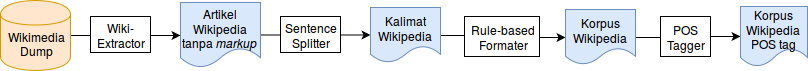
\includegraphics[width=\linewidth]{pics/Pic02-PreProcessingWikipedia}
    \caption{Pre-processing Data Wikipedia}
    \label{fig:preproses-wiki}
\end{figure}
Data hasi Wikipedia Dump diformat secara otomatis menggunakan \textit{tools} WikiExtractor. WikiExtractor adalah program berbasis Python yang dibuat oleh Giuseppe Attardi dan Antonio Fuschetto. Menggunakan \textit{tools} ini, didapatkan data yang sudah tidak mengikuti format MediaWiki Markup Language. Program ini dapat diunduh dari Github dan dijalankan menggunakan perintah berikut. 
\begin{lstlisting}[language=bash]
  $ WikiExtractor.py xml-dump-file -o output-file
\end{lstlisting}
Jika tidak memberi spesifikasi opsi apapun, artikel yang dihasilkan membersihkan seluruh markup language dan hanya menyimpan isi artikel tanpa disertakan informasi seperti kategori, riwayat, dan versi artikel.

%-----------------------------------------------------------------------------%
\subsection{Sentence Splitting}
%-----------------------------------------------------------------------------%
Korpus yang dihasilkan menghasilkan baris-baris yang merepresentasikan suatu paragraf dalam artikel Wikipedia. Pada penelitian kali ini, ingin dilihat relasi \textit{hypernym-hyponym} antar dua kata pada kalimat yang sama. Untuk itu, perlu dilakukan proses \textit{sentence splitting} yang dapat mengidentifikasi suatu kalimat dalam paragraf. Hasil dari proses tersebut adalah dokumen yang terdiri dari baris-baris yang merepresentasikan satu kalimat. 

Proses ini dilakukan dengan menggunakan \textit{script} yang telah dibuat sebelumnya oleh Ken Nabila Setya dari Fasilkom UI, Indonesia. Ditambah pula satu \textit{script} yang dapat secara otomatis melakukan \textit{splitting} untuk seluruh dokumen. Berikut adalah contoh sebuah paragraf dalam artikel Wikipedia yang telah dibersihkan menggunakan WikiExtractor.
\begin{center}
\begin{tabular}{ | m{32em} | } 
\hline
Charles Anthony Johnson (3 Juni 1829 - 17 Mei 1917), kemudian dikenal sebagai Charles Brooke memerintah Sarawak sebagai Raja Putih kedua dari 3 Agustus 1868 hingga meninggal dunia. Dia menggantikan pamannya, James Brooke sebagai raja. \\
\hline 
\end{tabular}
\end{center}

\noindent Setelah melalui proses \textit{sentence splitter}, berikut adalah hasilnya.
\begin{center}
\begin{tabular}{ | m{32em} | } 
\hline
Charles Anthony Johnson (3 Juni 1829 - 17 Mei 1917), kemudian dikenal sebagai Charles Brooke memerintah Sarawak sebagai Raja Putih kedua dari 3 Agustus 1868 hingga meninggal dunia. \\
\hline 
 Dia menggantikan pamannya, James Brooke sebagai raja. \\
\hline
\end{tabular}
\end{center}

%-----------------------------------------------------------------------------%
\subsection{Rule Based Formatter}
%-----------------------------------------------------------------------------%
Dari korpus yang berisi kalimat Wikipedia, diberikan beberapa aturan tambahan untuk membuat korpus sesuai format yang diinginkan. Penambahan aturan juga untuk mengurangi ambiguitas dan bentuk usaha generalisasi \textit{pattern}. Berikut adalah beberapa aturan tambahan untuk \textit{pre-processing} korpus Wikipedia.
\begin{enumerate}
  \item Menghilangkan frasa yang berada di dalam tanda kurung. \\
  Frasa yang terletak di dalam tanda kurung dapat dianggap sebagai penjelas kata atau frasa sebelumnya. Proses ini merupakan salah satu upaya generalisasi \textit{pattern}.
  \item Memisahkan simbol-simbol yang berhimpit pada awal dan akhir kata. \\
  Beberapa token yang dipisahkan oleh spasi dalam kalimat merupakan kata yang berhimpit dengan tanda baca. Untuk mempermudah proses selanjutnya yaitu \textit{sentence tagging}, dilakukan \textit{pre-processing} tambahan yaitu memisahkan simbol-simbol \textit{non-alphanumerical}.
  \item Memberi penanda awal kalimat dengan '<start>'' dan akhir kalimat dengan '<end>'. \\
  Pemberian simbol awal dan akhir kalimat memperjelas isi kalimat dan juga menunjang proses \textit{pattern extraction} dan \textit{pattern matching}.
\end{enumerate}

\noindent Dari contoh kalimat di atas, setelah melalui proses \textit{formatting} yang didefinisikan menghasilkan kalimat berikut.
\begin{center}
\begin{tabular}{ | m{32em} | } 
\hline
<start> Charles Anthony Johnson , kemudian dikenal sebagai Charles Brooke memerintah Sarawak sebagai Raja Putih kedua dari 3 Agustus 1868 hingga meninggal dunia . <end> \\
\hline 
<start> Dia menggantikan pamannya , James Brooke sebagai raja . <end> \\
\hline
\end{tabular}
\end{center}


%-----------------------------------------------------------------------------%
\section{POS Tagging Kalimat Wikipedia}
%-----------------------------------------------------------------------------%
Proses \textit{part-of-speech tagging} dilakukan pada korpus Wikipedia yang telah berbentuk kalimat dengan format yang didefinisikan. Pada penelitian ini, kelas kata yang menjadi pengamatan adalah \textit{noun} (NN) dan \textit{proper noun} (NNP), sehingga proses \textit{pos tagging} digunakan untuk identifikasi kata-kata tersebut. Proses \textit{pos tagging} menggunakan \textit{tools} Stanford POS Tagger, dengan model yang digunakan merupakan hasil penelitian sebelumnya menggunakan Bahasa Indonesia.  Setelah selesai melalui proses \textit{tagging}, dilakukan penyesuaian agar format korpus lebih rapi dan terstruktur. 

Berikut adalah contoh kalimat yang sudah melalui tahap \textit{pos tagging}. Korpus ini digunakan untuk proses \textit{pattern matching}.
\begin{center}
\begin{tabular}{ | m{32em} | } 
\hline
<start>\_X Charles\_NNP Anthony\_NNP Johnson\_NNP ,\_Z kemudian\_CC dikenal\_VB sebagai\_IN Charles\_NNP Brooke\_NNP memerintah\_VB Sarawak\_NNP sebagai\_IN Raja\_NNP Putih\_NNP kedua\_CD dari\_IN 3\_CD Agustus\_NNP 1868\_CD hingga\_IN meninggal\_VB dunia\_NN .\_Z <end>\_X \\ 
\hline
\end{tabular}
\end{center}


%-----------------------------------------------------------------------------%
\section{Seed Builder}
%-----------------------------------------------------------------------------%
\begin{figure}
    \centering
    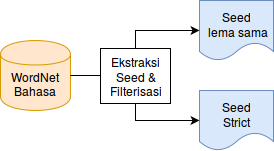
\includegraphics[scale=0.6]{pics/Pic02-SeedBuilder}
    \caption{Proses Pembentukan \textit{Seed}}
    \label{fig:seed-builder}
\end{figure}
Proses pengumpulan \textit{seed} dibantu dengan \textit{resource} yang dimiliki WordNet Bahasa menggunakan \textit{tools} nltk. Proses pengumpulan diawali dengan mengambil seluruh lema Bahasa Indonesia yang dimiliki oleh korpus nltk. Setelah itu, ambil seluruh \textit{synset} yang mengandung lemma tersebut. Dari setiap \textit{synset}, ambil relasi \textit{hypernym}-nya. Dari setiap \textit{synset} relasi, ambil lema Bahasa Indonesianya. Dilakukan pula filterisasi \textit{synset} ataupun lema untuk mengurangi ambiguitas. Untuk setiap \textit{synset} maupun lema yang diambil pada setiap tahapan, hanya boleh berasal dari kelas kata kerja (\textit{noun}). Setelah didapatkan, bentuk ke dalam pasangan \textit{tuple} 1-1 $(kata\_hyponym,kata\_hypernym)$.

%-----------------------------------------------------------------------------%
\subsection{Filterisasi Seed}
%-----------------------------------------------------------------------------%
Filterisasi dilakukan dengan tujuan mengurangi ambiguitas, namun tetap berusaha mendapatkan \textit{seed} sebanyak mungkin. Filterasisasi juga dilakukan untuk mendapatkan \textit{seed} awal yang diyakini benar dan berkualitas. Salah satu bagian terpenting proses ini adalah memasangkan hanya lema yang merupakan \textit{noun} ke lema yang juga adalah \textit{noun}. Jika kemungkinan lema tersebut tergolong ke dalam kelas kata bukan \textit{noun}, lema tidak diikutsertakan sebagai \textit{seed} awal.

Tantangan dalam proses ini adalah banyak ditemukan kasus dimana satu lema dikandung oleh lebih dari satu \textit{synset} atau satu \textit{synset} memiliki lebih dari satu \textit{synset hypernym}. Ambiguitas dalam kasus tersebut dapat mengurangi kualitas \textit{seed} yang dihasilkan. Mengatahui hal tersebut, dibuatlah dua pendekatan berbeda untuk proses filterisasi \textit{seed}.

Pendekatan pertama adalah tetap mengambil lemma yang sama pada \textit{synset hypernym} yang berbeda. Hal ini dilatarbelakangi adanya lema yang berasal dari \textit{synset} berbeda namun memiliki lema \textit{hypernym} yang sama. Pada contoh (i), satu lema yang sama dimiliki oleh dua \textit{synset} yang berbeda namun kedua \textit{synset} tersebut memiliki \textit{synset hypernym} yang sama. Lema untuk kedua \textit{synset hypernym} adalah sama sehingga tetap diikutsertakan sebagai \textit{seed}. Pada contoh (ii), satu lema berasal dari dua \textit{synset} yang berbeda dan dua \textit{synset hypernym} berbeda, namun ada lema yang sama yaitu 'laluan'.

Pendekatan lainnya adalah dengan metode filterisasi yang \textit{strict}. Jika satu lema memiliki lebih dari satu \textit{synset hypernym}, maka lema tersebut dianggap ambigu dan langsung tidak diikutsertakan ke dalam \textit{seed} awal. Berdasarkan tabel contoh lema, \textit{synset}, dan \textit{hypernym}-nya, hanya contoh (i) yang diterima sebagai \textit{seed} karena \textit{synset hypernym} untuk lema tersebut sama. Sementara (ii) ditolak karena \textit{synset hypernym} berbeda.

\begin{center}
\begin{tabular}{ |c|m{30em}| } 
\hline
\multirow{2}{*}{i.} & ('paruh', Synset('beak.n.02')) => (['bibir', 'kuala', 'muara'], [Synset('mouth.n.02')])
('paruh', Synset('beak.n.01')) => (['bibir', 'kuala', 'muara'], [Synset('mouth.n.02')]) \\ 
& ('paruh', Synset('beak.n.01')) => (['bibir', 'kuala', 'muara'], [Synset('mouth.n.02')]) \\ 
\hline
\multirow{2}{*}{ii.} & ('pintu\_masuk', Synset('entrance.n.01')) => (['akses', 'capaian', 'laluan'], [Synset('access.n.03')]) \\ 
& ('pintu\_masuk', Synset('orifice.n.01')) => (['koridor', 'laluan', 'lorong'], [Synset('passage.n.07')]) \\ 
\hline
\end{tabular}
\end{center}

%-----------------------------------------------------------------------------%
\subsection{Kelemahan Seed yang Dihasilkan}
%-----------------------------------------------------------------------------%
Walau sudah dilakukan proses filterisasi untuk meningkatkan kualitas \textit{seed}, masih ada hambatan yang belum bisa diatasi dalam penelitian ini. Beberapa kelemahan dari \textit{seed} awal yang dihasilkan adalah sebagai berikut.
\begin{itemize}
  \item \textit{Seed} yang mengandung kata bukan Bahasa Indonesia. Korpus yang ingin dibuat berdomain Bahasa Indonesia, namun \textit{seed} yang dihasilkan mengandung Bahasa Melayu atau Bahasa Indonesia lama. Beberapa kata bukan Bahasa Indonesia yang dihasilkan adalah 'had', 'bonjol', dan 'cecok'.
  \item Kesalahan semantik \textit{synset} dan lema Bahasa Indonesia. Beberapa \textit{synset} nltk memiliki lema Bahasa Indonesia yang kurang sesuai jika dilihat secara semantik. Sebagai contoh $Synset('scholar.n.01')$ dengan lemma Bahasa Indonesia ${'buku\_harian', 'pelajar'}$. Dalam Bahasa Indonesia, 'buku\_harian' memiliki makna yang berbeda dengan 'pelajar'.
  \item Kesalahan lema Bahasa Indonesia untuk suatu \textit{synset} menyebabkan dihasilkannya \textit{seed} yang jika dievaluasi kualitatif oleh manusia dirasa kurang tepat. Contoh \textit{seed} yang tidak baik adalah dari pemetaan $('sejarawan', Synset('historian.n.01')) => (['buku\_harian', 'pelajar'], [Synset('scholar.n.01')])$ dihasilkan \textit{seed} $(sejarawan,buku harian)$ dan $(sejarawan,pelajar)$. \textit{Seed} $(sejarawan,buku harian)$ adalah salah.
\end{itemize}


%-----------------------------------------------------------------------------%
\section{Sentence Tagging}
%-----------------------------------------------------------------------------%
Setelah memperoleh pasangan kata relasi Bahasa Indonesia, perlu dilakukan \textit{tagging} pasangan kata tersebut ke kalimat-kalimat dalam korpus Wikipedia. Data yang digunakan untuk proses ini adalah korpus Wikipedia tanpa \textit{pos tag}. Beberapa tahapan dilakukan pada proses \textit{tagging sentence} dengan pasangan kata relasi adalah sebagai berikut.
\begin{enumerate}
  \item Dibaca seluruh pasangan kata relasi \textit{hyponym-hypernym}.
  \item Untuk setiap kalimat pada korpus Wikipedia, di cek apakah kalimat tersebut mengandung pasangan kata relasi.
  \item Pengecekan dilakukan secara berulang untuk seluruh pasangan kata relasi karena terdapat kemungkinan satu kalimat mengandung lebih dari satu pasang kata relasi.
  \item Kata-kata yang merupakan bagian dari pasangan kata relasi kemudian di-\textit{tag} sesuai relasinya dan disimpan ke dalam korpus berisi kalimat dengan \textit{tag} \textit{hyponym} dan \textit{hypernym}.
\end{enumerate}
Pada penelitian ini, satu kalimat yang telah di-\textit{tag} hanya mengandung tepat satu pasangan kata relasi. Untuk kasus khusus dimana suatu pasangan kata relasi terdiri dari satu kata yang merupakan sub kata pasangannya, maka pasangan kata tersebut tidak diikutsertakan untuk menghindari ambiguitas. Contoh pasangan kata yang tidak diikutsertakan adalah $(ikan\,\,gurame;ikan)$, kata 'ikan' terkandung dalam kedua kata relasi. 

Berikut adalah contoh kalimat yang terbentuk dari proses \textit{sentence tagging}. Diberikan pasangan kata relasi \textit{hyponym-hypernym} $(fermion;partikel)$ dan $(boson;partikel)$ serta kalimat  '<start> seluruh partikel dasar adalah boson atau fermion . <end>'. Hasil proses \textit{sentence tagging} adalah sebagai berikut.
\begin{center}
\begin{tabular}{ | m{32em} | } 
\hline
<start> seluruh <hypernym>partikel<hypernym> dasar adalah boson atau <hyponym>fermion<hyponym> . <end> \\ 
\hline
<start> seluruh <hypernym>partikel<hypernym> dasar adalah <hyponym>boson<hyponym> atau fermion . <end> \\ 
\hline
\end{tabular}
\end{center}

\begin{figure}
    \centering
    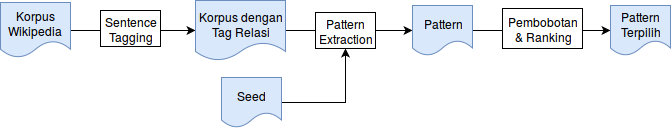
\includegraphics[width=\linewidth]{pics/Pic03-PatternExtraction}
    \caption{Proses Pembentukan \textit{Pattern}}
    \label{fig:pattern-extraction}
\end{figure}

%-----------------------------------------------------------------------------%
\section{Pattern Extraction}
%-----------------------------------------------------------------------------%
Setelah mendapatkan kalimat-kalimat yang telah di-\textit{tag} dengan kata relasi, ingin dicari \textit{pattern} yang dapat digunakan untuk menambah jumlah relasi kata. Pembuatan \textit{pattern} menggunakan algoritma dasar \textit{standard trie} dengan beberapa modifikasi. Proses ini diimplementasi secara mandiri menggunakan program Java dengan mengikuti algoritma pembuatan \textit{Trie} sederhana.

Suatu \textit{\textit{node}} merepresentasikan kata dalam kalimat dan dari satu kalimat terbentuk sebuah cabang dalam \textit{tree}. \textit{Node} menyimpan beberapa informasi seperti nama \textit{\textit{node}}, \textit{parent}, \textit{childs}, dan informasi identitas tambahan seperti apakah \textit{\textit{node}} tersebut merupakan relasi (\textit{hypernym} atau \textit{hyponym}) dan apakah \textit{\textit{node}} tersebut merupakan \textit{leaf}. Untuk kata yang merupakan kata relasi, \textit{\textit{node}} menyimpan informasi jenis relasi beserta \textit{list} dari kata yang merupakan bagian dari relasi tersebut. 

\noindent Sebagai contoh dua kalimat sebagai berikut.
\begin{center}
\begin{tabular}{ | m{32em} | } 
\hline
<start> <hyponym>singa<hyponym> adalah <hypernym>kucing<hypernym> yang berukuran besar <end> \\ 
\hline
\hline
<start> <hyponym>serigala<hyponym> adalah <hypernym>anjing<hypernym> yang tinggal di hutan <end>\\ 
\hline
\end{tabular}
\end{center}

\noindent Akan menghasilkan \textit{Pattern} Tree sebagai berikut. Angka setelah kata adalah bobot suatu \textit{node}.
\begin{lstlisting}[language=bash]
`-^ (1)
 `-<hyponym> (2)
   `-adalah (2)
     `-<hypernym> (2)
       `-yang (2)
        |-berukuran (1)
        | `-besar (1)
        `-tinggal (1)
          `-di (1)
            `-hutan (1)
\end{lstlisting}

%-----------------------------------------------------------------------------%
\subsection{Informasi dalam Pattern}
%-----------------------------------------------------------------------------%
Beberapa informasi yang disimpan dalam suatu \textit{pattern} adalah \textit{sequence} kata yang merepresentasikan \textit{pattern} tersebut, jumlah kemunculan dalam korpus, \textit{seed} unik yang membentuk \textit{pattern}, dan kalimat unik yang membentuk \textit{pattern}. Informasi-informasi tersebut digunakan untuk pembentukan vektor \textit{pattern}, pemberian bobot \textit{pattern} dan melakukan \textit{sorting} untuk mendapatkan \textit{pattern} terbaik.

%-----------------------------------------------------------------------------%
\subsection{Pattern Tree}
%-----------------------------------------------------------------------------%
\textit{Pattern Tree} adalah sebuah \textit{tree} yang menyimpan seluruh \textit{pattern} yang dihasilkan dari korpus. Dalam pembuatan \textit{pattern tree}, tidak perlu menyimpan seluruh kata dalam kalimat. Hanya \textit{sequence} kata tertentu saja yang dianggap dapat menghasilkan \textit{pattern} yang baik untuk diikutsertakan. Maka dari itu, perlu diambil \textit{sequence} kata dalam kalimat yang digunakan sebagai \textit{pattern}. Terdapat tiga pendekatan dalam proses ini, diantaranya adalah sebagai berikut.
\begin{enumerate}
  \item Hanya memperhatikan kata yang berada diantara pasangan kata relasi. \\
  Pada kasus ini, hanya ingin dilihat kata-kata yang berada diantara kata yang merupakan \textit{hypernym-hyponym} atau \textit{hyponym-hypernym}. Kata-kata diantara dua relasi dapat dianggap paling dekat jika ingin mencari \textit{pattern} relasi tersebut. Pada contoh diatas, \textit{sequence} kata yang dihasilkan adalah '<hyponym>singa<hyponym> adalah <hypernym>kucing<hypernym>'
  \item Mengikutsertakan $n$ kata sebelum kata relasi pertama. \\
  Beberapa kata sebelum kata relasi, dapat memberikan informasi untuk yang dapat meningkatkan kualitas \textit{pattern} yang dihasilkan. Pada contoh diatas dengan $(n=1)$, \textit{sequence} kata yang dihasilkan adalah '<start> <hyponym>singa<hyponym> adalah <hypernym>kucing<hypernym>'
  \item Mengikutsertakan $n$ kata setelah kata relasi terakhir. \\
  Tipe ini sama dengan sebelumnya, namun dilihat pengaruh kata-kata yang mengikuti kata relasi. Pada contoh diatas dengan $(n=1)$, \textit{sequence} kata yang dihasilkan adalah '<hyponym>singa<hyponym> adalah <hypernym>kucing<hypernym> yang'
\end{enumerate}

%-----------------------------------------------------------------------------%
\subsection{Vektor Pattern}
%-----------------------------------------------------------------------------%
Suatu \textit{pattern} dapat direpresentasikan menjadi vektor berdasarkan nilai-nilai yang dimilikinya. Vektor ini dapat dimanfaatkan untuk menentukan \textit{pattern} yang baik (pembobotan). Fitur utama pada vektor \textit{pattern} diambil dari informasi yang disimpan oleh suatu \textit{pattern}, yaitu total kemunculan \textit{pattern}, jumlah \textit{seed} unik, dan jumlah kalimat unik yang membentuk \textit{pattern} tersebut. Fitur lain adalah hasil kombinasi perbandingan antar nilai utama. Fitur tambahannya adalah nilai perbandingan antara jumlah \textit{seed} unik dibagi jumlah kalimat unik, nilai perbandingan antara jumlah \textit{seed} untuk dibagi total kemunculan, dan nilai perbandingan antara jumlah kalimat unik dibagi total kemunculan.

%-----------------------------------------------------------------------------%
\subsection{Validasi dan Filterisasi Pattern}
%-----------------------------------------------------------------------------%
Setelah terbentuk \textit{pattern tree}, perlu di-\textit{list} seluruh \textit{pattern} yang dihasilkan. Proses pembentukan \textit{pattern} cukup dengan menelusuri \textit{path} dari \textit{\textit{node} leaf} hingga \textit{root}. Untuk mengurangi \textit{pattern} yang kurang baik, dilakukan proses validasi. Beberapa aturan yang harus dipenuhi agar suatu \textit{pattern} dianggap \textit{valid} adalah sebagai berikut.
\begin{itemize}
  \item Harus ada minimal satu kata diantara dua kata relasi. \\
  Banyak kasus dimana dua kata relasi hanya dipisahkan oleh spasi. \textit{Pattern} yang hanya mengandung spasi tidak memberikan informasi apapun karena simbol spasi dalam Bahasa Indonesia digunakan sebagai pemisah antar kata. Sebagai contoh kalimat hasil tagging '<start> semua jenis <hypernym>ular<hypernym> <hyponym>beludak<hyponym> memiliki taring yang panjang <end>' tidak akan menghasilkan \textit{pattern} yang \textit{valid}.
  \item Sebuah \textit{pattern} harus memenuhi nilai \textit{threshold} yang didefinisikan. Nilai perbandingan antara jumlah \textit{seed} unik dibagi jumlah kalimat unik lebih dari 0.5. Nilai perbandingan antara jumlah \textit{seed} unik dibagi total kemunculan lebih dari 0.2. Nilai perbandingan antara jumlah kalimat unik dibagi total kemunculan harus lebih dari 0.7. Ketiga nilai \textit{threshold} tersebut didefinisikan sendiri berdasarkan pengamatan nilai pada vektor \textit{pattern}.
\end{itemize}

%-----------------------------------------------------------------------------%
\subsection{Pembentukan \textit{Pattern} Unik}
%-----------------------------------------------------------------------------%
\textit{Pattern} yang dihasilkan dari tahap ini harus unik sehingga tidak terjadi ambiguitas jika hendak digunakan. Pada masa awal pengembangan, masalah yang muncul pada \textit{pattern} yang dihasilkan adalah adanya \textit{pattern} yang posisi penempatan \textit{hypernym-hyponym}-nya saling berkebalikan. Sebagai contoh beberapa \textit{pattern} ambigu yang dihasilkan seperti (i) <hyponym> adalah <hypernym>, (ii) <hypernym> adalah <hyponym>, (iii) <hypernym> dan <hyponym>, dan (iv) <hyponym> dan <hypernym>. Padahal, bagian \textit{hypernym-hyponym} tersebut nantinya digantikan dengan kata yang kemunculannya cocok dengan \textit{pattern} yang diberikan. Jika \textit{pattern} tersebut dibiarkan begitu saja, akan banyak dihasilkan \textit{pair} yang salah.

Strategi yang dilakukan untuk masalah ambiguitas antar \textit{pattern} adalah membangun suatu arsitektur yang dapat mengidentifikasi dan menyelesaikannya. Tahapan pembangunan \textit{pattern} unik adalah sebagai berikut.
\begin{enumerate}
  \item Dicari \textit{pattern} dengan pendekatan hanya memperhatikan kata-kata diantara pasangan kata relasi.
  \item \textit{Pattern} yang dihasilkan dievaluasi satu dengan yang lain. Jika terdapat \textit{pattern} yang saling terbalik, \textit{pattern} yang bersangkutan dikeluarkan dari \textit{list} dan disimpan untuk dievaluasi ulang.
  \item Proses evaluasi ulang dilakukan menggunakan pendekatan pembuatan \textit{pattern} lainnya yaitu, memperhatikan $n$ kata sebelum atau sesudah kemunculan relasi.
  \item Hasil kedua pendekatan digabung dan dicek apakah \textit{pattern} tersebut dibutuhkan. Suatu \textit{pattern} hasil evaluasi ulang dinyatakan dibutuhkan jika \textit{substring} dari \textit{pattern} tersebut tergolong dalam \textit{list pattern} yang membutuhkan evaluasi ulang.
  \item Proses evaluasi dilakukan secara berulang dari dengan $n$ yang terus bertambah dari 1 (satu). Pada penelitian ini nilai $n$ dibatasi hingga 2 (dua), sehingga maksimum ada dua kata sebelum kata relasi pertama atau dua kata setelah kata relasi terakhir.
\end{enumerate}

Setelah melakukan tahapan di atas, tidak ada lagi kasus posisi relasi saling tertukar dari \textit{pattern} yang dihasilkan. \textit{List pattern} yang dihasilkan kemudian diurutkan sebelum ditampilkan.

%-----------------------------------------------------------------------------%
\subsection{Pengurutan Pattern}
%-----------------------------------------------------------------------------%
Setelah didapatkan \textit{pattern} yang sesuai, dilakukan proses pengurutan (\textit{sorting}) untuk mengetahui \textit{pattern} mana yang terbaik berdasarkan bobot yang dimiliki. Proses pengurutan dilakukan dengan membandingkan satu \textit{pattern} dengan yang lain, dengan tahapan sebagai berikut.
\begin{enumerate}
  \item Semakin besar jumlah kalimat unik yang membentuk \textit{pattern}.
  \item Semakin besar nilai perbandingan antara jumlah \textit{seed} unik yang membentuk \textit{pattern} dengan jumlah kalimat unik yang membentuk \textit{pattern}.
  \item Semakin kecil jumlah token dalam \textit{pattern} tersebut jika di-\textit{parse} dengan spasi.
\end{enumerate}

%-----------------------------------------------------------------------------%
\subsection{Kelemahan Pattern yang Dihasilkan}
%-----------------------------------------------------------------------------%
Hasil dari tahap ekstraksi \textit{pattern} dengan aturan-aturan di atas diharapkan memberi \textit{pattern} yang baik untuk merepresentasikan relasi kata \textit{hyponym-hypernym}. Namun, proses ini tidak terlepas dari beberapa masalah. Salah satu hambatan yang belum dapat diselesaikan seperti menentukan \textit{pattern} mana yang lebih baik jika satu \textit{pattern} adalah \textit{substring} dari \textit{pattern} yang lain. Selain itu, proses generalisasi \textit{pattern} juga belum dapat diimplementasi. 

Beberapa \textit{pattern} terlihat kurang baik secara semantik jika dilihat secara kualitatif. \textit{Pattern} seperti (a) <hypernym> dan <hyponym>, (b) <hypernym> atau <hyponym> kurang cocok jika digunakan dalam \textit{pattern matching}. Hal ini disebabkan kata 'dan' dan 'atau' memuat relasi yang bersifat simetris. Sementara \textit{hypernym-hyponym} merupakan relasi yang hanya memiliki sifat transitif. Pada penelitian ini, relasi yang diamati hanya \textit{hypenym-hyponym}. Namun ada kemungkinan suatu \textit{pattern} yang sama dapat digunakan untuk relasi semantik berbeda dan mungkin lebih cocok digunakan utnuk relasi lain tersebut. Tidak adanya perbandingan \textit{pattern} yang dihasilkan oleh relasi semantik lain menjadi salah satu hambatan memilih \textit{pattern} yang baik.


%-----------------------------------------------------------------------------%
\section{Pattern Matching}
%-----------------------------------------------------------------------------%
\textit{Pattern} yang terbentuk dari proses \textit{pattern extraction} digunakan untuk menambah jumlah pasangan kata relasi dengan dilakukan proses \textit{pattern matching} terhadap korpus Wikipedia. Proses \textit{Pattern} Matching menggunakan algoritma \textit{Suffix Tree} dengan modifikasi. Implementasi dilakukan secara mandiri menggunakan program Java.

\begin{figure}
    \centering
    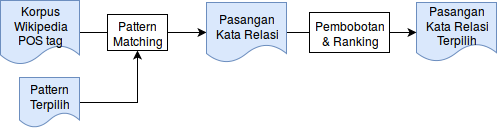
\includegraphics[scale=0.6]{pics/Pic04-PatternMatching}
    \caption{Proses Pembentukan \textit{Pair}}
    \label{fig:pattern-matching}
\end{figure}

Sebuah \textit{node} merepresentasikan satu kata dalam kalimat. Untuk setiap kalimat, dibentuk sebuah suffix tree yang merepresentasikan kalimat tersebut dan selanjutnya dicocokan dengan \textit{pattern} yang ada. Dibuat pula kelas \textit{Pair} yang merepresentasikan pasangan kata relasi \textit{hypernym-hyponym} yang dihasilkan dari proses \textit{pattern matching}. \textit{Pair} menyimpan informasi seperti total kemunculan, total dokumen unik, daftar kalimat unik dan \textit{pattern} unik yang menghasilkan \textit{pair}.

Tahapan proses \textit{pattern matching} jika diberikan satu kalimat dan satu \textit{pattern} adalah sebagai berikut.
\begin{enumerate}
  \item Kalimat masukan dibentuk menjadi suatu \textit{suffix tree}.
  \item \textit{Pattern} masukan ditokenisasi ke dalam bentuk \textit{list} kata. \textit{Pattern} pasti mengandung token <hypernym> dan <hyponym>, selanjutnya disebut token relasi.
  \item Jika ditemukan token relasi pada \textit{list pattern} yang sedang dievaluasi, maka \textit{node} yang dikunjungi disimpan sementara sesuai dengan relasinya.
  \item Jika token bukan token relasi, maka di evaluasi apakah token sama dengan \textit{node} yang dikunjungi. Jika sama maka proses evaluasi dilanjutkan, namun jika berbeda maka \textit{pattern} tidak cocok.
  \item Jika seluruh token \textit{pattern} telah dievaluasi dan tidak mengalami kegagalan, makan dianggap berhasil dan kata yang terekstrak disimpan dalam bentuk \textit{pair}.
\end{enumerate}

Pada masa awal pengembangan, setelah dijalankan proses \textit{pattern matching} terhadap korpus Wikipedia dengan \textit{pattern} hasil ekstraksi, masalah pertama yang ditemukan adalah banyaknya \textit{pair} yang salah satu atau kedua kata relasinya tidak teramasuk dalam kelas kata benda. Beberapa \textit{pair} yang salah diantaranya $(Menoitios;salah)$ dimana 'salah' adalah \textit{adjective} dan $(saya,gitaris)$ dimana 'saya' adalah preposi. Untuk itu diputuskan menggunakan korpus Wikipedia yang sudah melalui tahap POS Tagging.

Masalah lain yang muncul adalah jika kata yang ingin diekstrak merupakan \textit{multi word}. \textit{Pair} kurang baik yang dihasilkan sebelum mengatasi masalah ini diantaranya $(bola;olahraga)$ yang seharusnya $(sepak\,\,bola;olahraga)$, $(Serikat;negara)$ yang seharusnya $(Amerika\,\,Serikat;negara)$, dan $(Monterrey,ibu)$ yang seharusnya $(Monterrey;ibu\,\,kota)$. Solusi yang digunakan untuk mengatasi masalah ini adalah dengan mengasumsikan kata-kata berurutan yang memiliki kelas kata sama dalam suatu kalimat merupakan \textit{multi word}. \textit{Multi word} disimpan dalam satu \textit{node} pada pembentukan \textit{suffix tree}.

%-----------------------------------------------------------------------------%
\subsection{Vektor Pair}
%-----------------------------------------------------------------------------%
Suatu \textit{pair} dapat direpresentasikan ke dalam bentuk vektor berdasarkan nilai-nilai yang dimilikinya. Nilai-nilai fitur yang dimiliki oleh sebuah \textit{pair} adalah total kemunculan \textit{pair}, total dokumen yang membentuk \textit{pair}, jumlah \textit{pattern} unik, dan jumlah kalimat unik. Untuk memperkaya fitur \textit{pair}, dilakukan pula Word Embedding. Nilai \textit{similarity} antar dua kata relasi ditambahkan sebagai sebagai salah satu fitur.

%-----------------------------------------------------------------------------%
\subsection{Filterisasi dan Validasi Pair}
%-----------------------------------------------------------------------------%
\textit{Pair} baru yang dihasilkan untuk proses ini berjumlah sangat banyak, namun tidak semua \textit{pair} yang dihasilkan memenuhi relasi \textit{hypernym-hyponym}. Beberapa \textit{pair} kebetulan terekstrak akibat memenuhi \textit{pattern} lekscal yang sama dengan salah satu \textit{pattern} yang digunakan untuk proses \textit{pattern matching}. Untuk mengeliminasi data yang tidak diyakini benar, dilakukan validasi sederhana untuk setiap \textit{pair} yang dihasilkan. \textit{Pair} dinyatakan benar jika terdapat lebih dari satu \textit{pattern} yang mengekstrak \textit{pair} tersebut.

Setelah mengeliminasi \textit{pair} yang hanya terbentuk dari satu \textit{pattern}, dilakukan pembobotan. Tidak semua \textit{pair} yang dihasilkan masuk ke dalam korpus kata relasi. Bobot satu \textit{pair} dihitung menggunakan rumus berikut. 
\[ Bobot = (\frac{jumlah\,\,pattern\,\,pembentuk\,\,pair}{jumlah\,\,pattern\,\,digunakan} + similarity\,\,score)/2 \]
\noindent Jika nilai bobot melebihi threshold, maka \textit{pair} dimasukan ke dalam korpus pasangan kata relasi.

%-----------------------------------------------------------------------------%
%\subsection{Pengurutan Pair}
%-----------------------------------------------------------------------------%
%Pada saat ditampilkan, \textit{pair} diurutkan untuk mengetahui \textit{pair} mana yang diyakini paling benar. Proses pengurutan dilakukan berdasarkan beberapa tahap, yaitu:
% Semakin besar jumlah \textit{pattern} unik yang menghasilkan \textit{pair}.
% Semakin besar jumlah kalimat untuk yang menghasilkan \textit{pair}.


%-----------------------------------------------------------------------------%
\subsection{Pemodelan Word Embedding}
%-----------------------------------------------------------------------------%
Untuk menambah fitur pada vektor \textit{pair} yang dapat menunjang proses evaluasi, dilakukan Word Embedding. Implementasinya menggunakan model Word2Vec berbasis Python. Proses ini dibuat secara otomatis dengan hanya mengmasukan dokumen Bahasa Indonesia berukuran besar. Dalam penelitian ini, dokumen Bahasa Indoensia yang digunakan adalah korpus Wikipedia yang telah di proses.

Model dibuat menggunakan korpus Wikipedia yang telah melalui proses POS Tagging. Korpus tersebut diolah sedemikian sehingga kata-kata yang dianggap \textit{multi word}, memiliki kelas kata sama berurutan, digabung dengan simbol garis bawah ('\_'). Hal ini dilatarbelakangi atas hasil \textit{pair} yang banyak merupakan \textit{multi word}. Jika hal ini tidak dilakukan, maka akan banyak kata yang tidak ditemukan dalam \textit{dictionary} yang dihasilkan \textit{model word embedding}.

Model yang terbentuk, digunakan untuk memberi nilai \textit{similarity} antara kata \textit{hypernym-hyponym} dalam satu \textit{pair}. Hal ini diharapkan dapat memberi informasi lebih mengenai kualitas \textit{pair} yang dihasilkan.

%%-----------------------------------------------------------------------------%
\chapter{\babLima}
%-----------------------------------------------------------------------------%

%-----------------------------------------------------------------------------%
\section{Implementasi \f{Cluster}}
%-----------------------------------------------------------------------------%

%-----------------------------------------------------------------------------%
\subsection{Instalasi \f{Frontend}}
%-----------------------------------------------------------------------------%
Tabel model lain, ditunjukkan pada tabel \ref{tab:infohasti}. 
\begin{table}
	\centering
	\caption{Informasi \f{cluster} X}
	\newcolumntype{g}{>{\columncolor{headertbl}}c}
	\label{tab:infohasti}
	\begin{tabular}{|g|c|}
	\hline Host Name & X\\
	\hline Cluster Name & X\\
	\hline Certificate Organization & UI\\
	\hline Certificate Locality & Depok\\
	\hline Certificate State & West Java\\
	\hline Certificate Country & ID\\
	\hline Contact & X\\
	\hline URL & http://grid.ui.ac.id\\
	\hline
	\end{tabular}
\end{table}

Ada pagebreak disini.
%supaya rapih
\pagebreak

Another type of table
\begin{table}
	\centering
	\caption{Perbandingan Partisi \f{default} dan manual}
	\newcolumntype{g}{>{\columncolor{headertbl}}c}
	\label{tab:partdisk}
	\begin{tabular}{|g|c|c|}
	\rowcolor{headertbl}
	\hline & Partisi default & Partisi manual yang dilakukan\\
	\hline / & 16 GB & 30 GB\\
	\hline /var & 4 GB & 18 GB\\
	\hline swap & 1 GB & 2 GB\\
	\hline /export & 55 GB & 26 GB\\
	\hline
	\end{tabular}
\end{table}

Program menghasilkan keluaran seperti pada kode \ref{lst:raidready}. 

\begin{minipage}{\linewidth}
\begin{lstlisting}[caption={Keluaran output},label={lst:raidready}]
[root@nas-0-0 ~]# cat /proc/mdstat 
Personalities : [raid1] 
md0 : active raid1 sda4[0] sdb2[1]
      1917672312 blocks super 1.2 [2/2] [UU]
      
unused devices: <none>
[root@nas-0-0 ~]# mdadm --detail /dev/md0 
/dev/md0:
        Version : 1.2
  Creation Time : Fri May  3 15:38:52 2013
     Raid Level : raid1
     Array Size : 1917672312 (1828.83 GiB 1963.70 GB)
  Used Dev Size : 1917672312 (1828.83 GiB 1963.70 GB)
   Raid Devices : 2
  Total Devices : 2
    Persistence : Superblock is persistent

    Update Time : Tue May 28 11:27:49 2013
          State : clean 
 Active Devices : 2
Working Devices : 2
 Failed Devices : 0
  Spare Devices : 0

           Name : nas-0-0.local:0  (local to host nas-0-0.local)
           UUID : 0754726d:3dfbd4b9:42b0f587:68631556
         Events : 28

    Number   Major   Minor   RaidDevice State
       0       8        4        0      active sync   /dev/sda4
       1       8       18        1      active sync   /dev/sdb2
\end{lstlisting}
\end{minipage}

%-----------------------------------------------------------------------------%
\subsection{Konfigurasi}\label{cha:confcluster}
%-----------------------------------------------------------------------------%
Contoh verbatim dalam itemize : 
\begin{itemize}
\item \bo{Bold ini}\\
dijalankan perintah berikut : 
\begin{Verbatim}[frame=single]
# javac Ganteng.java
# java Ganteng
\end{Verbatim}
\paragraph{}
Perilaku sistem 
\begin{Verbatim}[frame=single]
# hai
# enable
# cd /export/rocks/install/
# create distro
# sh sesuatu.sh
# reboot
\end{Verbatim}
\paragraph{}

\item \bo{Menambahkan \f{package} pada \f{compute node}}\\
Langkah yang dilakukan adalah sebagai berikut : 
	\begin{enumerate}
	\item Masuk ke dalam direktori \co{/procfs/}
	\item Membuat/Mengubah berkas \co{xx.xml}. Jika tidak terdapat berkas tersebut, dapat disalin dari \co{skeleton.xml}.
	\item Menambahkan \f{package} yang ingin dipasang pada \f{compute node} diantara \f{tag} \co{<package>} seperti berikut : \co{<package>[package yang akan dipasang]</package>}.
	\item Menjalankan perintah berikut termasuk perintah untuk melakukan instalasi ulang seluruh \f{compute node}: 
	\begin{Verbatim}[frame=single]
# cd /export/somedir
# create
# run host
	\end{Verbatim}
	\end{enumerate}
	\paragraph{}
\end{itemize}
%-----------------------------------------------------------------------------%
\subsubsection{semakin ke dalam}
%-----------------------------------------------------------------------------%
\begin{minipage}{\linewidth}
\begin{lstlisting}[caption={Keluaran mentah untuk detail \f{job}}, label={lst:outqstatf},style=L]
[ardhi@xx ~]$ qstat -f 138
Job Id: 138.xx
    Job_Name = cur-1000-1np
    Job_Owner = ardhi@xx
    resources_used.cput = 27:21:35
    resources_used.mem = 86060kb
    resources_used.vmem = 170440kb
    resources_used.walltime = 27:24:50
    job_state = R
    queue = default
    server = hastinapura.grid.ui.ac.id
    Checkpoint = u
    ctime = Fri May 31 10:27:37 2013
    Error_Path = xx:/home/ardhi/xx/curcumin-1000/cur-1000-1np.e138
    exec_host = compute-0-5/0
    exec_port = 15003
    Hold_Types = n
    Join_Path = n
    Keep_Files = n
    Mail_Points = e
    Mail_Users = ardhi.putra@ui.ac.id
    mtime = Fri May 31 10:27:47 2013
    Output_Path = xx:/home/ardhi/xx/curcumin-1000/cur-1000-1np.o138
    Priority = 0
    qtime = Fri May 31 10:27:37 2013
    Rerunable = True
    Resource_List.nodes = 1:ppn=1
    session_id = 5768
    etime = Fri May 31 10:27:37 2013
    submit_args = cur-1000-1np.pbs
    start_time = Fri May 31 10:27:47 2013
    submit_host = xx
    init_work_dir = /home/ardhi/xx/curcumin-1000   
\end{lstlisting}
\end{minipage}

%-----------------------------------------------------------------------------%
\section{Pengujian} %lebih ke gimana cara ujinya
%-----------------------------------------------------------------------------%

%-----------------------------------------------------------------------------%
\subsection{Kasus Uji}
%-----------------------------------------------------------------------------%
Berwarna!
\begin{lstlisting}[caption=Potongan skrip submisi \f{job} melalui torqace,label={lst:grotorqace},style=shell]
# Go To working directory
cd $PBS_O_WORKDIR

#openMPI prerequisite
. /opt/torque/etc/openmpi-setup.sh

mpirun -np 5 -machinefile $PBS_NODEFILE mdrun -v -s \ 
	curcum400ps.tpr -o md_prod_curcum400_5np.trr -c lox_pr.gro
...
\end{lstlisting}
%-----------------------------------------------------------------------------%
\subsection{Kasus Uji}
%-----------------------------------------------------------------------------%
Contoh skrip yang dimasukkan pada \f{form} yang disediakan dapat dilihat pada kode \ref{lst:makebzip}.
\begin{lstlisting}[caption={Potongan \co{Makefile} \f{project}}, label={lst:makebzip},style=shell]
# Make file for MPI
SHELL=/bin/sh

# Compiler to use
# You may need to change CC to something like CC=mpiCC
# openmpi : mpiCC
# mpich2  : /opt/mpich2/gnu/bin/mpicxx
CC=mpiCC
...
...
\end{lstlisting}
%%-----------------------------------------------------------------------------%
\chapter{\babEnam}
%-----------------------------------------------------------------------------%

%-----------------------------------------------------------------------------%
\section{Hasil Pengujian}
%-----------------------------------------------------------------------------%
%-----------------------------------------------------------------------------%
\subsection{Hasil Pengujian Kasus Uji 1}
%-----------------------------------------------------------------------------%
Tabel lain. Hasil tersebut dapat dilihat pada tabel \ref{tab:hasilgrrd}.
\begin{table}
	\centering
	\caption{Hasil pengujian menggunakan gromacs}
	\label{tab:hasilgrrd}
	\begin{tabular}{|c|l|*{3}{c|}}
		\rowcolor{headertbl}
  		\hline % create horizontal line
  		No & \f{Timestep} & \multicolumn{3}{|>{\columncolor{headertbl}}c|}{Waktu eksekusi berdasar jumlah prosesor} \\
		\hhline{|>{\arrayrulecolor{headertbl}}*{2}{-}>{\arrayrulecolor{black}}*{3}{|-|}}
  		\rowcolor{headertbl} & & 1 & 2 & 5 \\
  		\hline 1 & 200ps & 20h:27m:16s & 12h:59m:04s & 5h:07m:03s \\
  		\hline 2 & 400ps & 1d:22h:40m:03s & 1d:02h:08m:47s & 10h:09m:39s \\
  		\hline 3 & 600ps & 2d:23h:29m:21s & 1d:14h:52m:52s & 15h:25m:22s \\
  		\hline 4 & 800ps & 4d:02h:05m:57s & 2d:03h:30m:07s & 20h:29m:38s \\
  		\hline 5 & 1000ps & 5d:03h:29m:12s & 2d:16h:32m:22s & 1d:01h:34m:38s \\
  		\hline
	\end{tabular}
\end{table}
%-----------------------------------------------------------------------------%
\section{Evaluasi Hasil Kasus Uji}
%-----------------------------------------------------------------------------%
%-----------------------------------------------------------------------------%
\subsection{Evaluasi Kasus Uji 1}
%-----------------------------------------------------------------------------%
Tabel \ref{tab:hasilgrrd} menunjukkan hasil uji coba pada penelitian ini.  Gambar \ref{fig:grafgro5} menunjukkan perbandingan waktu eksekusi pada aplikasi x dengan jumlah prosesor sebanyak 5 buah.

\begin{figure}
	\centering
	\includegraphics[width=1\textwidth]
		{pics/5np-gromacs-chart.pdf}
	\caption{Perbandingan waktu eksekusi x untuk 5 prosesor}
	\label{fig:grafgro5}
\end{figure}
\paragraph{}
%%-----------------------------------------------------------------------------%
\chapter{\babTujuh}
%-----------------------------------------------------------------------------%
Pada bab terakhir ini, 
%---------------------------------------------------------------
\section{Kesimpulan}
%---------------------------------------------------------------

%---------------------------------------------------------------
\section{Saran}
%---------------------------------------------------------------


%\printbibliography
%
% Daftar Pustaka
%\include{pustaka}
%biblama (bukan biblatex)
\bibliography{bib}{}
%\bibliography{references}{}
%biblama (bukan biblatex)
\bibliographystyle{apalikerd}
%\bibliographystyle{ieeetr} 

%
% Lampiran 
%
%\begin{appendix}
%	%
% @author  Andreas Febrian
% @version 1.00 
% 
% Hanya sebuah pembatas bertuliskan LAMPIRAN ditengah halaman. 
% 

\begin{titlepage}
	\centering 
	\vspace*{6cm}
	\noindent \Huge{LAMPIRAN}
	\addChapter{LAMPIRAN}
\end{titlepage} 
%	\setcounter{page}{2}
%	%-----------------------------------------------------------------------------%
\addChapter{Lampiran 1 : Pattern Buatan Manual}
\chapter*{Lampiran 1 : Pattern Buatan Manual}
%-----------------------------------------------------------------------------%
Berikut adalah daftar \textit{pattern} yang dibentuk secara manual oleh anotator.
\begin{itemize}
  \item <hypernym> adalah kumpulan dari <hyponym>
  \item <hypernym> antara lain adalah <hyponym>, <hyponym>, dan <hyponym>
  \item <hypernym> dapat dibedakan menjadi <hyponym>
  \item <hypernym> lainnya, seperti <hyponym> dan <hyponym>
  \item <hypernym> seperti <hyponym>
  \item <hypernym> terdiri dari <hyponym>, <hyponym>, dan <hyponym>
  \item <hypernym> terdiri dari beberapa bagian, seperti <hyponym>, <hyponym>, dan <hyponym>
  \item <hypernym> terutama <hyponym> yang
  \item <hypernym>, khususnya <hyponym>, adalah
  \item <hypernym>, misalnya <hyponym>
  \item <hypernym>, misalnya <hyponym> dan <hyponym>
  \item <hypernym>, terutama <hyponym>, adalah
  \item <hyponym> adalah <hypernym>
  \item <hyponym> adalah <hypernym> dari
  \item <hyponym> adalah <hypernym> dengan
  \item <hyponym> adalah <hypernym> yang berhubungan dekat dengan <hyponym>
  \item <hyponym> adalah <hypernym> yang bersifat
  \item <hyponym> adalah bagian dari <hypernym> yang
  \item <hyponym> adalah salah satu <hypernym>
  \item <hyponym> adalah sebuah <hypernym> yang
  \item <hyponym> adalah sejenis <hypernym> dengan
  \item <hyponym> adalah suatu <hypernym>
  \item <hyponym> atau <hyponym> adalah suatu jenis <hypernym> yang
  \item <hyponym> berarti <hypernym>
  \item <hyponym> dan <hyponym> dianggap sebagai <hypernym>
  \item <hyponym> dan <hyponym> merupakan <hypernym> yang
  \item <hyponym> dan berbagai <hyponym> lainnya adalah <hypernym> yang
  \item <hyponym> dan sejumlah <hyponym> lainnya termasuk ke dalam kategori <hypernym>
  \item <hyponym> dapat digolongkan ke dalam <hypernym>
  \item <hyponym> dapat dimasukkan ke dalam kategori <hypernym> dan <hypernym>
  \item <hyponym> dianggap sebagai <hypernym> karena
  \item <hyponym> dikenal juga sebagai <hypernym>
  \item <hyponym> disebut sebagai <hypernym> yang
  \item <hyponym> ialah <hypernym>
  \item <hyponym> menjadi <hypernym> apabila
  \item <hyponym> menjadi <hypernym> yang
  \item <hyponym> menjadi salah satu bagian dari <hypernym> karena
  \item <hyponym> merujuk pada <hypernym>
  \item <hyponym> merujuk pada <hypernym> yang
  \item <hyponym> merupakan <hypernym>
  \item <hyponym> merupakan <hypernym> yang
  \item <hyponym> merupakan suatu <hypernym> yang
  \item <hyponym> secara khusus menjadi sebutan bagi <hypernym> yang
  \item <hyponym> termasuk <hypernym> yang
  \item <hyponym> termasuk ke dalam <hypernym> yang
  \item <hyponym> termasuk ke dalam kategori <hypernym>
  \item <hyponym> termasuk ke dalam salah satu <hypernym> yang
  \item <hyponym> tersebut merupakan <hypernym>
  \item Beberapa <hypernym> seperti <hyponym>
  \item Beberapa contoh <hypernym> lainnya adalah <hyponym>
  \item Beberapa jenis dari <hypernym> adalah <hyponym> dan <hyponym>
  \item Berbagai <hypernym> seperti <hyponym>
  \item Contoh dari <hypernym> adalah <hyponym>
  \item Contoh dari <hypernym>, yaitu <hyponym>, <hyponym>, dan <hyponym>
  \item Istilah umum dari <hyponym> adalah <hypernym>
  \item Jenis <hypernym> yang paling banyak dikenal adalah <hyponym>
  \item Jenis-jenis <hypernym> antara lain <hyponym> dan <hyponym>
  \item Salah satu <hypernym> adalah <hyponym>
  \item Salah satu <hypernym> yang mirip dengan <hyponym> adalah <hyponym>
  \item Salah satu contoh dari <hypernym> adalah <hyponym>
  \item Sebagai salah satu <hypernym>, <hyponym>
  \item Sebagai sebuah <hypernym>, <hyponym> merupakan
  \item Secara umum, <hyponym> merupakan <hypernym> yang dapat
  \item Selain <hyponym>, <hyponym> juga menjadi <hypernym> yang
  \item Terdapat banyak <hypernym>, seperti <hyponym>
  \item Terdapat beberapa contoh <hypernnym>, di antaranya <hyponym>, <hyponym>, dan <hyponym>
  \item Walaupun <hyponym> adalah <hypernym>, tetapi 
\end{itemize}

%-----------------------------------------------------------------------------%
\addChapter{Lampiran 2 : Panduan Pembuatan dan Anotasi Pattern}
% \chapter*{Lampiran 2 : Panduan Pembuatan danaa Anotasi Pattern}
%-----------------------------------------------------------------------------%
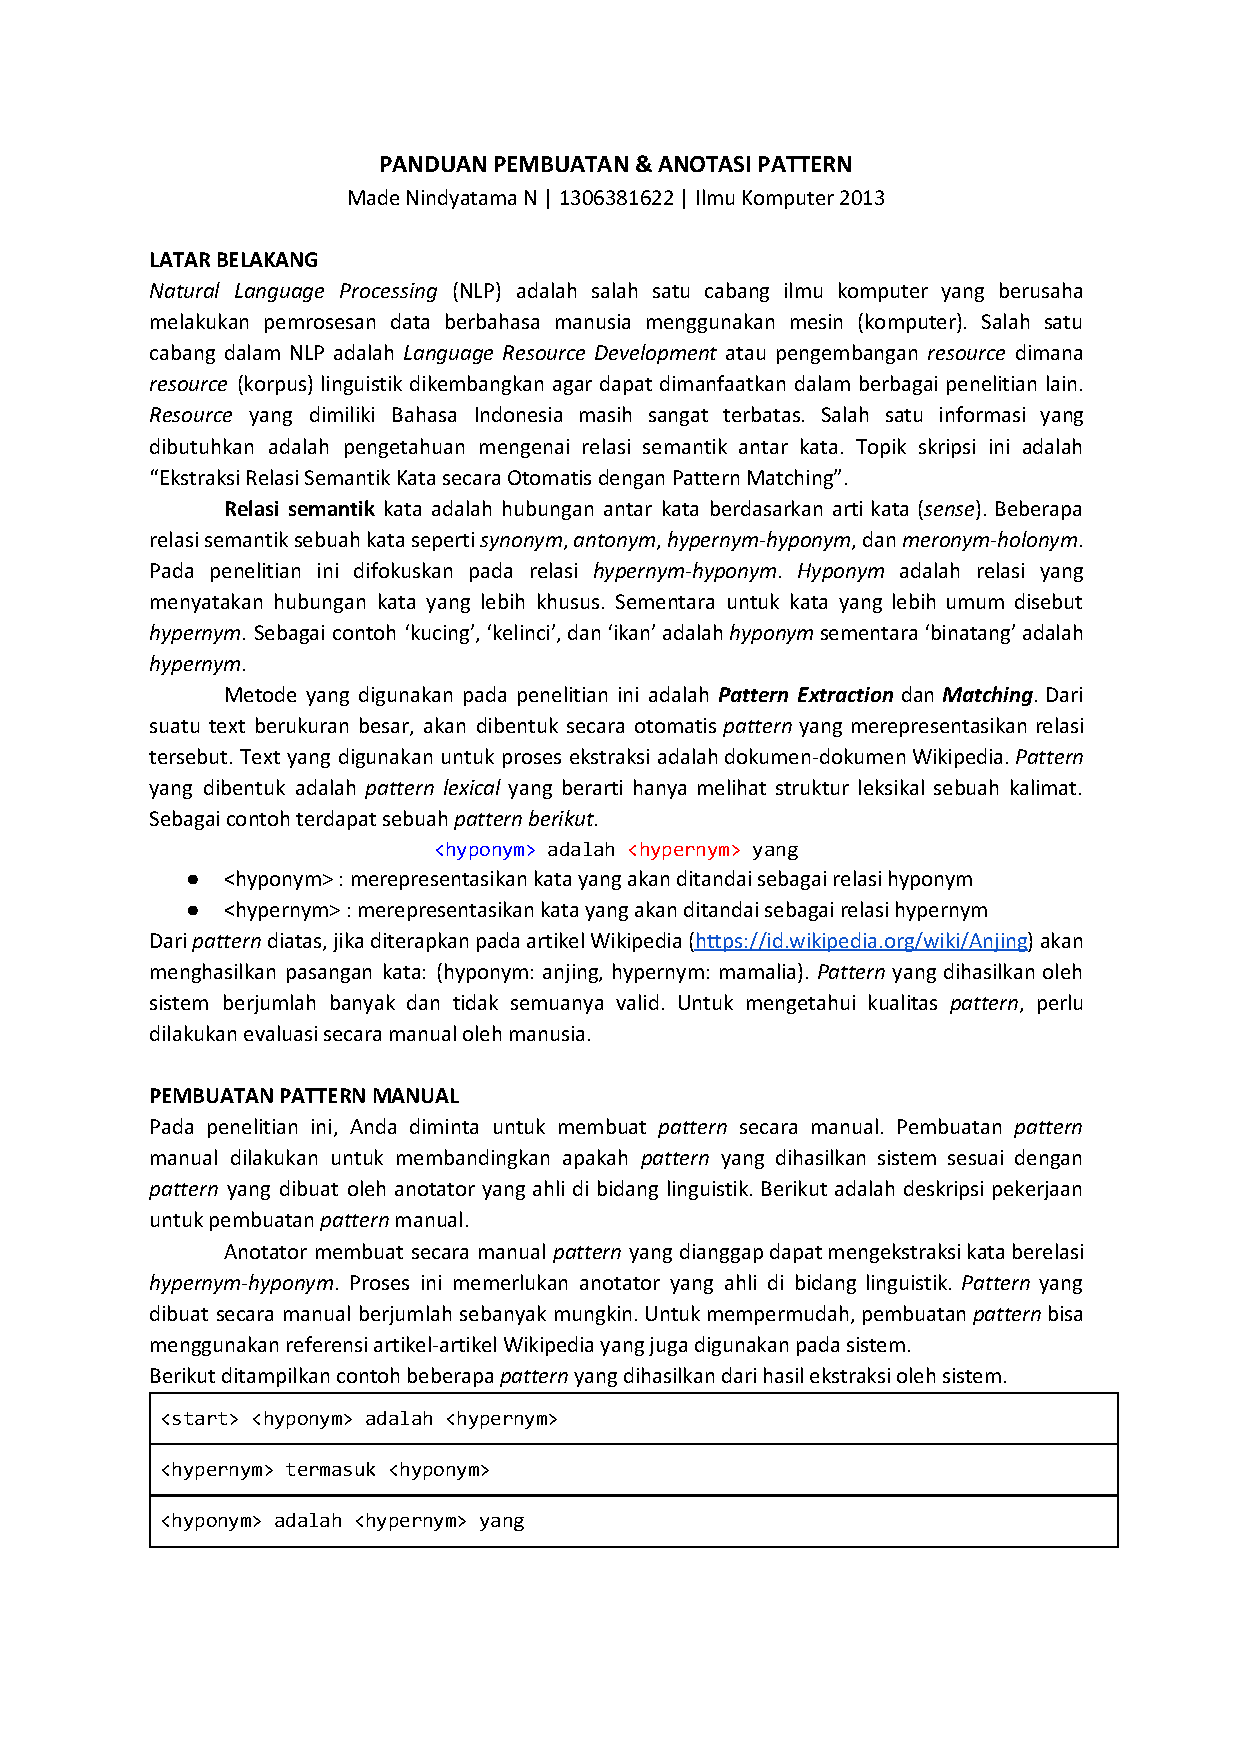
\includepdf[pages={1}]{PanduanPembuatanAnotasiPattern.pdf}
\includepdf[pages={2}]{PanduanPembuatanAnotasiPattern.pdf}

%-----------------------------------------------------------------------------%
\addChapter{Lampiran 3 : Panduan Anotasi Pair}
%-----------------------------------------------------------------------------%
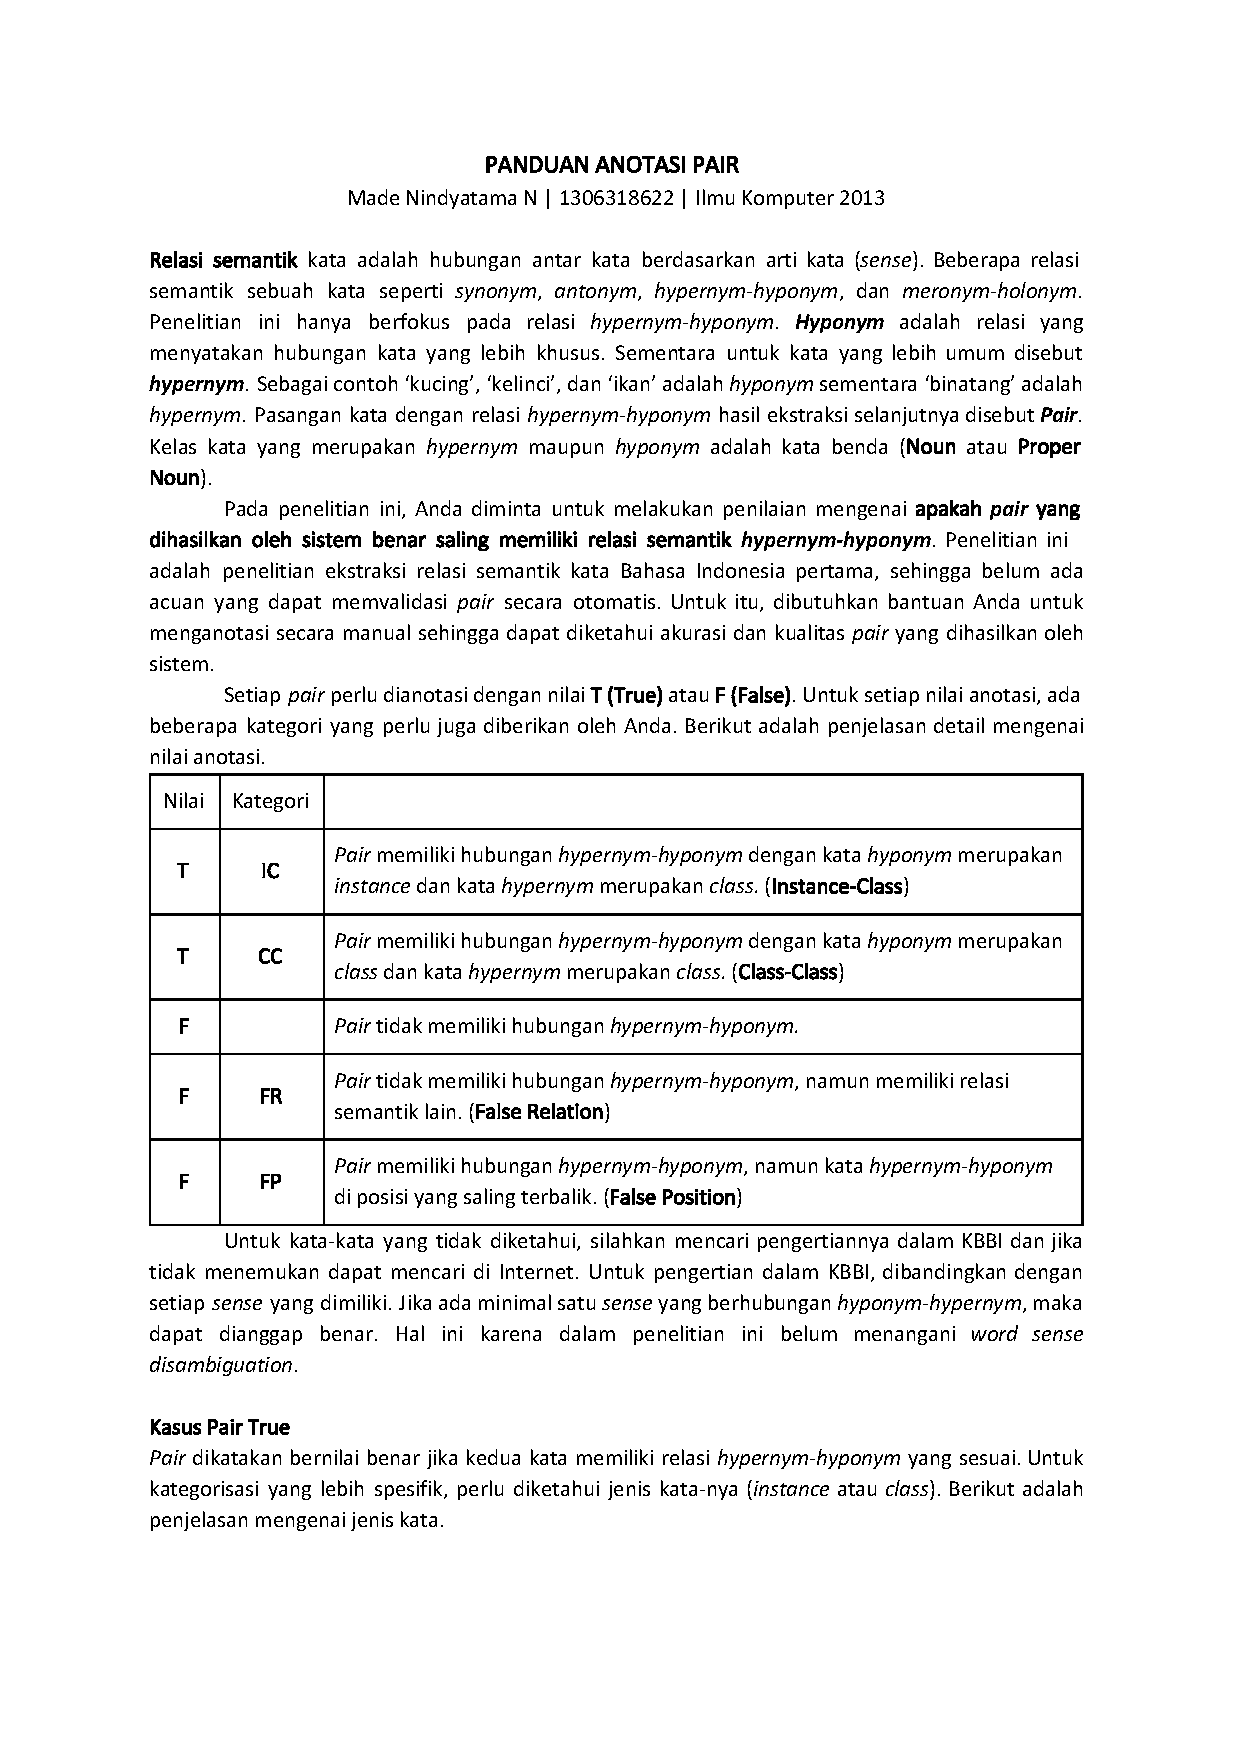
\includepdf[pages={1}]{PanduanAnotasiPair.pdf}
\includepdf[pages={2}]{PanduanAnotasiPair.pdf}
\includepdf[pages={3}]{PanduanAnotasiPair.pdf}

% \section*{\code{admin\_useraddmaster}} \label{cha:lampir-admin}
% Skrip ini diletakkan pada direktori \co{/usr/sesuatu} dan hanya dapat dieksekusi oleh \f{root}. Skrip ini berguna untuk menambahkan pengguna baru sesuai dengan konfigurasi baru yang telah ditetapkan.
% \begin{lstlisting}[style=L,caption={Skrip menambahkan pengguna baru},label={lst:adduser}]
% #!/bin/csh -f
% blah blah blah
% blah blah blah
% blah blah blah
% blah blah blah
% blah blah blah
% \end{lstlisting}

% \section*{\code{getuser.cron}} \label{cha:lampir-cronadmin}
% Penjelasan skrip disini
% \begin{lstlisting}[style=L,caption={\f{Cronjob} menambahkan pengguna baru},label={lst:cronadduser}]
% #!/bin/bash
% # Change these two lines to localize to your system:
% # Adapted from /usr/local/sbin/admin_useradd

% cat /dev/null > $userlist
% for (( i=0; i<${#listemailto[@]}; i++ ))
% do
%         uname=${listusername[$i]}
%         mailto=${listemailto[$i]}

%         echo "User $uname created, please use torqace wisely." | mail -s "Torqace user registration" $mailto
% done

% \end{lstlisting}
% 
% %-----------------------------------------------------------------------------%
% \addChapter{Lampiran 2 : Berkas Konfigurasi}
% \chapter*{Lampiran 2 : Berkas Konfigurasi}
% %-----------------------------------------------------------------------------%
% \section*{compute.xml}
% \begin{lstlisting}[caption={Berkas \co{compute.xml}},label={lst:excomp},language=XML]
% <?xml version="1.0" standalone="no"?>
% <kickstart>
% <description>
% 	Compute node XML file
% </description>
% </kickstart> 
% \end{lstlisting}

% %-----------------------------------------------------------------------------%
% \addChapter{Lampiran 8 : UAT dan Kuesioner}
% %-----------------------------------------------------------------------------%
% \begin{landscape}
% \chapter*{Lampiran 8 : UAT dan Kuesioner}
% \begin{longtable}{|c|p{7cm}|p{2.5cm}|p{3.5cm}|p{3.3cm}|p{1.8cm}|}
% \caption{Tabel UAT dan Kuesioner} \label{tab:uattbl}\\
% \hline
% No. & \multicolumn{1}{c|}{Langkah Penggunaan} & Fitur Berjalan & Tingkat Kemudahan (1-5) & Tingkat Kepuasan (1-5) & Saran / Komentar \\ 
% \cline{3-5} & & Berhasil /Tidak & 1:Sangat sulit ; \hspace{100pt} 5:sangat mudah & 1 : Sangat kecewa ; 5 : sangat puas &  \\ \hline
% \multicolumn{ 6}{|>{\columncolor{headertbl}}c|}{Use Case : Login} \\ \hline
% 1.1 & Pengguna berada pada halaman depan torqace &  &  &  &  \\ \hline
% 1.2 & Pengguna memasukkan username dan password pada field yang telah disediakan.Kemudian menekan tombol 'login' &  &  &  &  \\ \hline
% 1.3 & Apabila Sukses, maka pengguna masuk ke dalam sistem dan dihadapkan pada menu utama &  &  &  &  \\ \hline
% \multicolumn{ 6}{|>{\columncolor{headertbl}}c|}{Use Case : Register} \\ \hline
% 2.1 & Pengguna berada pada halaman registrasi pengguna torqace &  &  &  &  \\ \hline
% 2.2 & Pengguna memasukkan username,password, dan email pada field yang telah disediakan. Kemudian menekan tombol 'submit' &  &  &  &  \\ \hline
% 2.3 & Sistem akan mengonfirmasi masukan, dan akan mengirimkan email untuk memberitahu pengguna apabila proses pendaftaran telah selesai &  &  &  &  \\ \hline
% \multicolumn{ 6}{|>{\columncolor{headertbl}}c|}{Use Case : Logout} \\ \hline
% 3.1 & Pengguna memilih menu untuk melakukan logout &  &  &  &  \\ \hline
% 3.2 & Sistem akan mengeluarkan pengguna, dan pengguna tidak dapat menggunakan fitur-fitur utama aplikasi &  &  &  &  \\ \hline
% \multicolumn{ 6}{|>{\columncolor{headertbl}}c|}{Use Case : Upload Job Sederhana} \\ \hline
% 4.1 & Pengguna memilih menu upload file/project pada menu utama &  &  &  &  \\ \hline
% 4.2 & Pengguna memilih pilihan 'single file' pada tipe project &  &  &  &  \\ \hline
% 4.3 & Pengguna memilih berkas yang akan diunggah, mengisi label, dan menentukan apakah akan menimpa project sebelumnya dengan nama yang sama atau tidak &  &  &  &  \\ \hline
% 4.4 & Pengguna menekan tombol 'submit' dan mengonfirmasi  &  &  &  &  \\ \hline
% 4.5 & Sistem akan menampilkan informasi terkait berkas yang diupload &  &  &  &  \\ \hline
% \multicolumn{ 6}{|>{\columncolor{headertbl}}c|}{Use Case : Upload Job Compressed} \\ \hline
% 5.1 & Pengguna memilih menu upload file/project pada menu utama &  &  &  &  \\ \hline
% 5.2 & Pengguna memilih pilihan 'compressed files' pada tipe project &  &  &  &  \\ \hline
% 5.3 & Pengguna memilih arsip yang akan diunggah, mengisi label, menentukan akan melakukan make atau tidak dan menentukan apakah akan menimpa project sebelumnya dengan nama yang sama atau tidak &  &  &  &  \\ \hline
% 5.4 & Pengguna menekan tombol 'submit' dan mengonfirmasi  &  &  &  &  \\ \hline
% 5.5 & Sistem akan menampilkan informasi terkait berkas yang diupload dan diekstrak. Keluaran make juga akan ditampilkan bila dipilih &  &  &  &  \\ \hline
% \multicolumn{ 6}{|>{\columncolor{headertbl}}c|}{Use Case : Upload Array Job} \\ \hline
% 6.1 & Pengguna memilih menu upload file/project pada menu utama &  &  &  &  \\ \hline
% 6.2 & Pengguna memilih pilihan 'array' pada tipe project &  &  &  &  \\ \hline
% 6.3 & Pengguna memilih arsip-arsip yang akan diunggah, mengisi label, menentukan akan melakukan make atau tidak dan menentukan apakah akan menimpa project sebelumnya dengan nama yang sama atau tidak &  &  &  &  \\ \hline
% 6.4 & Pengguna menekan tombol 'submit' dan mengonfirmasi  &  &  &  &  \\ \hline
% 6.5 & Sistem akan menampilkan informasi terkait berkas yang diupload dan diekstrak. Keluaran make juga akan ditampilkan bila dipilih &  &  &  &  \\ \hline
% \multicolumn{ 6}{|>{\columncolor{headertbl}}c|}{Use Case : Melihat antrian pada queue} \\ \hline
% 7.1 & Pengguna memilih menu  queue status pada menu utama &  &  &  &  \\ \hline
% 7.2 & Pengguna berada pada halaman yang berisi informasi queue &  &  &  &  \\ \hline
% \multicolumn{ 6}{|>{\columncolor{headertbl}}c|}{Use Case : Melihat detil antrian} \\ \hline
% 8.1 & Dari halaman status queue, pengguna memilih job tertentu &  &  &  &  \\ \hline
% 8.2 & Informasi mengenai detil job tersebut ditampilkan dalam bentuk tabel &  &  &  &  \\ \hline
% 8.2.1 & Apabila job tersebut bukan milik pengguna, maka sistem akan melarang pengguna melihat informasi detil suatu job &  &  &  &  \\ \hline
% \multicolumn{ 6}{|>{\columncolor{headertbl}}c|}{Use Case : Membuat script job} \\ \hline
% 9.1 & Pengguna memilih untuk melakukan 'generate script' baik dari laporan upload berkas, atau dari penjelajahan direktori &  &  &  &  \\ \hline
% 9.2 & Pengguna mengisi nama job, parameter job, dan script yang akan dijalankan.  &  &  &  &  \\ \hline
% 9.3 & Pengguna mengonfirmasi konfirmasi submit job &  &  &  &  \\ \hline
% 9.4 & Pengguna dapat melihat informasi script secara keseluruhan dan pesan apakah terjadi kegagalan atau tidak, serta id job yang diberikan &  &  &  &  \\ \hline
% \multicolumn{ 6}{|>{\columncolor{headertbl}}c|}{Use Case : Load spesifikasi job lain} \\ \hline
% 10.1 & Pengguna berada pada halaman untuk membuat script &  &  &  &  \\ \hline
% 10.2 & Pengguna memilih 'Load a Previous Job' &  &  &  &  \\ \hline
% 10.3 & Pengguna memilih job mana yang akan dimuat dan menekan tombol 'Load' &  &  &  &  \\ \hline
% 10.4 & Pengguna kembali ke halaman pembuatan script dengan spesifikasi job sebelumnya &  &  &  &  \\ \hline
% \multicolumn{ 6}{|>{\columncolor{headertbl}}c|}{Use Case : Menjelajah Direktori} \\ \hline
% 11.1 & Pengguna memilih menu  'View File/Project'  pada menu utama &  &  &  &  \\ \hline
% 11.2 & Pengguna dapat melakukan navigasi untuk masuk ke dalam direktori tertentu, atau kembali ke direktori diatasnya, dan dapat melihat terdapat berkas apa saja dalam direktori &  &  &  &  \\ \hline
% \multicolumn{ 6}{|>{\columncolor{headertbl}}c|}{Use Case : Menghapus Berkas/Direktori} \\ \hline
% 12.1 & Pengguna berada pada halaman penjelajahan direktori &  &  &  &  \\ \hline
% 12.2 & Pengguna memilih pilihan untuk menghapus berkas/direktori di samping item yang akan dihapus &  &  &  &  \\ \hline
% 12.3 & Pengguna mengonfirmasi konfirmasi penghapusan &  &  &  &  \\ \hline
% \multicolumn{ 6}{|>{\columncolor{headertbl}}c|}{Use Case : Mengunduh Berkas/Direktori} \\ \hline
% 13.1 & Pengguna berada pada halaman penjelajahan direktori &  &  &  &  \\ \hline
% 13.2 & Pengguna memilih pilihan untuk mengunduh berkas/direktori di samping item yang akan dihapus &  &  &  &  \\ \hline
% \multicolumn{ 6}{|>{\columncolor{headertbl}}c|}{Use Case : Melihat Berkas} \\ \hline
% 14.1 & Pengguna berada pada halaman penjelajahan direktori &  &  &  &  \\ \hline
% 14.2 & Pengguna memilih berkas yang berupa berkas teks &  &  &  &  \\ \hline
% 14.3 & Sistem akan menampilkan konten dari berkas tersebut &  &  &  &  \\ \hline
% \end{longtable}
% \end{landscape}

%\end{appendix}

\end{document}
